% Created 2017-12-14 jeu. 14:42
% Intended LaTeX compiler: pdflatex
\documentclass[10pt,svgnames,fragile]{beamer}
\usepackage[frenchb]{babel}
\usepackage[utf8x]{inputenc}
\usepackage{lmodern}
\usepackage[T1]{fontenc}
\usepackage{graphicx}
\usepackage{etex}
\usepackage{xcolor}
\usepackage[normalem]{ulem}
\usepackage{textcomp}
\usepackage{pdflscape}
\usepackage{marvosym}
\usepackage{wasysym}
\usepackage{amssymb}
\usepackage{amsmath}
\usepackage{amsthm}
\usepackage{qtree}
\usepackage{bussproofs}
\usepackage{proof}
\usepackage{fitch}
\usepackage{cancel}
\usepackage{url}
\usepackage{smfthm}
\usepackage{animate}
\usepackage{cite}
\usepackage{caption}
\usepackage{hyperref}
\usepackage{tikz}
\usepackage{xcolor} % To add color
\AtBeginSection[]{\begin{frame}<beamer>\frametitle{}\tableofcontents[currentsection,hideothersubsections]\end{frame}}
\subtitle{}
\institute[]{SOTA Report: \newline Hyperspectral Image Analysis for  Cluster Detection}
\titlegraphic{
\includegraphics[height=2.5cm]{duke}}
\usetheme{CambridgeUS}
\usepackage{beamer_udl_theme}
\setbeamertemplate{navigation symbols}{}
\author{Juntang Wang}
\date{}
\title{Group Meeting May 30, 2024}
\begin{document}
\maketitle

\section{Definition and Problem Description}
\begin{frame}{Introduction - HSI \& Unsupervised Clustering}
    \begin{columns}
        % Left column
        \begin{column}{0.38\textwidth}
            \begin{figure}
            \centering
            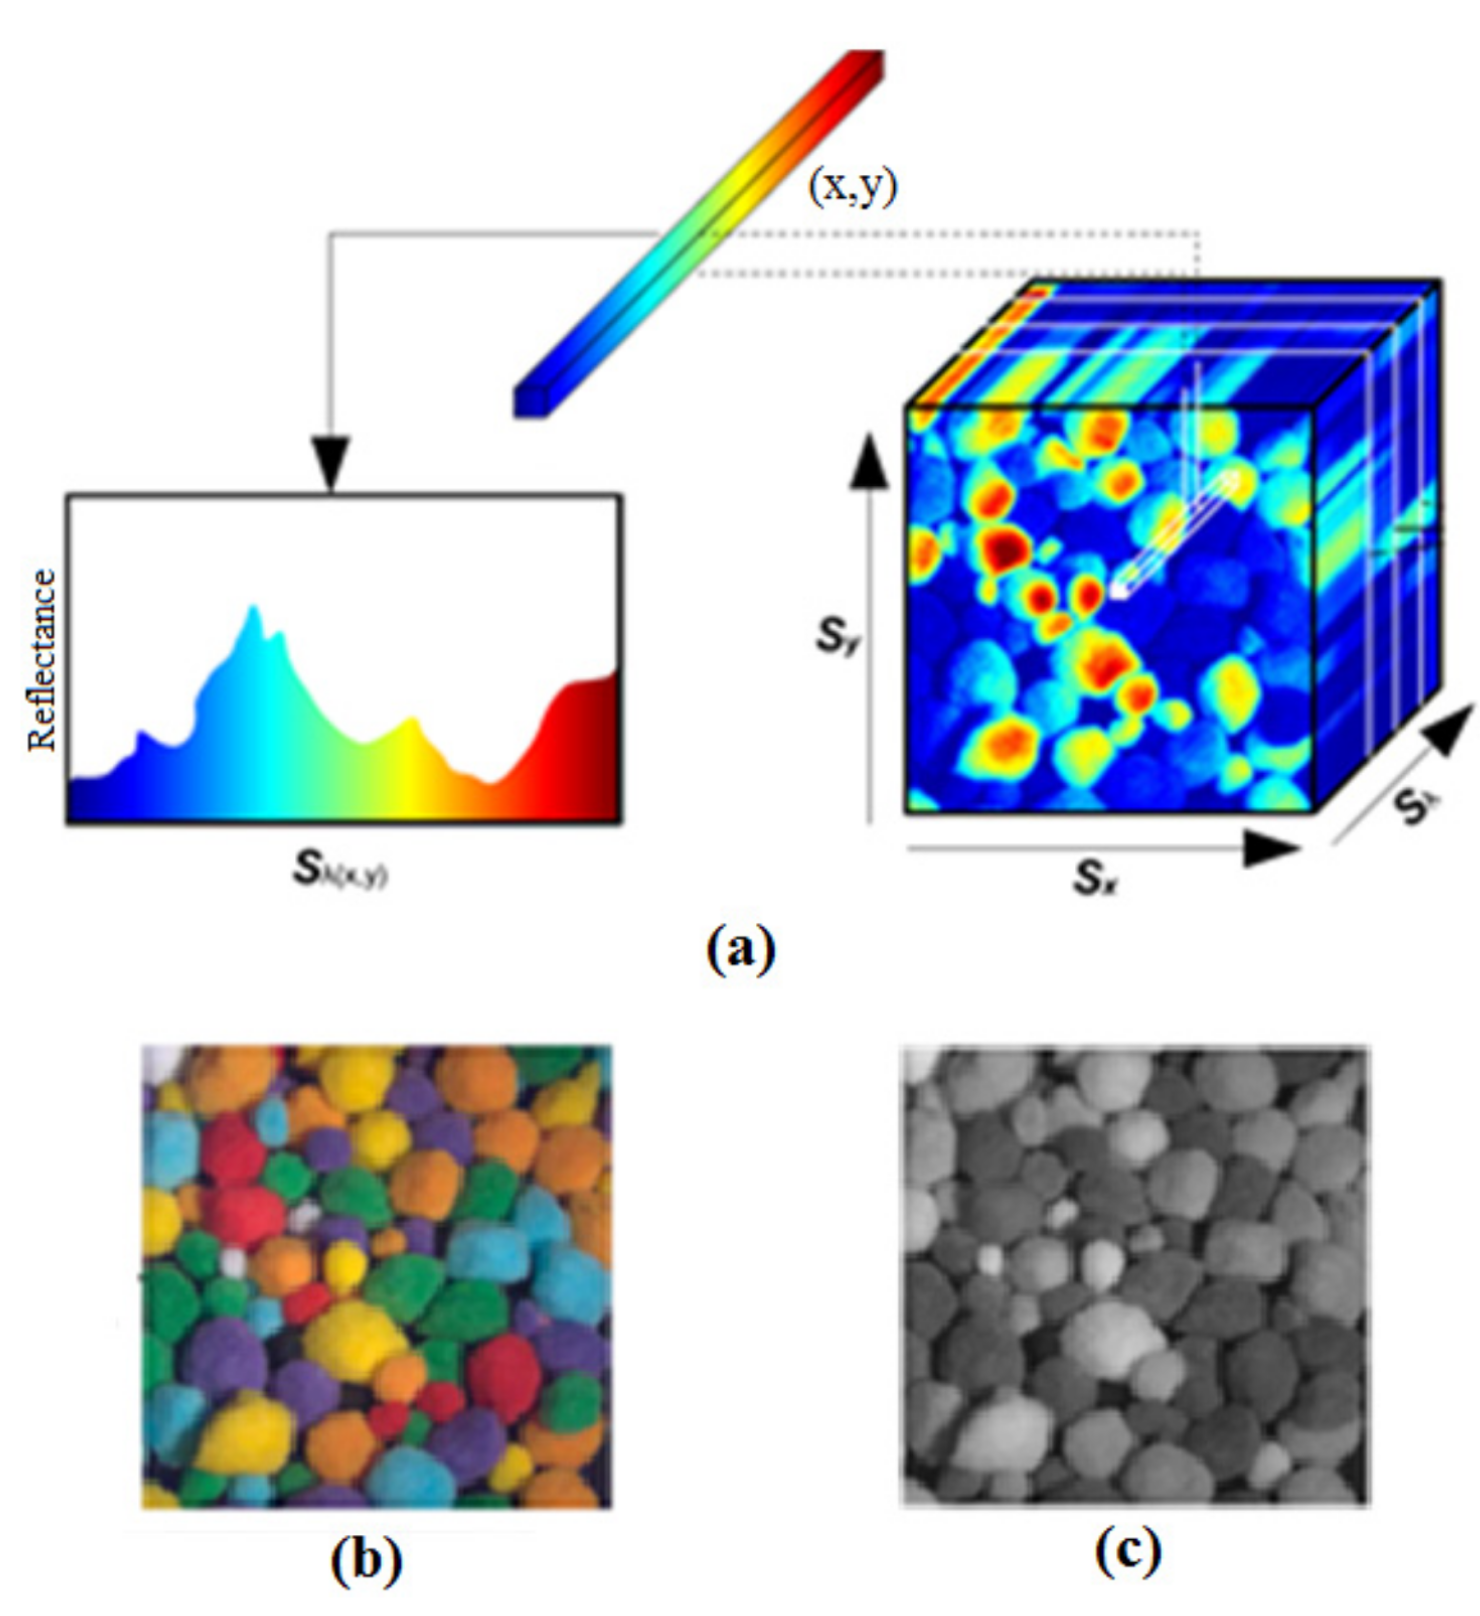
\includegraphics[width=1\linewidth]{HSI_example.png}
            \captionsetup{labelformat=simple, labelsep=colon, font=tiny, labelfont={color=gray,bf}}
            \caption{(a) A hyperspectral image represented as a 3D cube. A point spectrum on the spectral cube is illustrated at the spatial location (x,y). (b) An RGB image and (c) a grayscale image rendered from the hyperspectral cube.\cite{khanModernTrendsHyperspectral2018}}
            \label{fig:khan-modern}
            \end{figure}
        \end{column}

        % Right column
        \begin{column}{0.62\textwidth}
            \begin{itemize}
                \item \small \textbf{Hyperspectral Imaging (HSI)} is a technique that captures image data at multiple wavelengths across the electromagnetic spectrum, providing detailed spectral information for each pixel.
                \item \small \textbf{Unsupervised Clustering} involves grouping pixels in HSI data without prior labels, identifying natural structures and patterns in the data.
                \item \small By applying unsupervised clustering to HSI, we aim to detect distinct materials and features within images, enhancing applications in agriculture, remote sensing, and medical diagnostics.
            \end{itemize}
        \end{column}
    \end{columns}
\end{frame}

\begin{frame}{The Problem to Address}
    \begin{columns}
        % Left column
        \begin{column}{0.38\textwidth}
            \begin{figure}
            \centering
            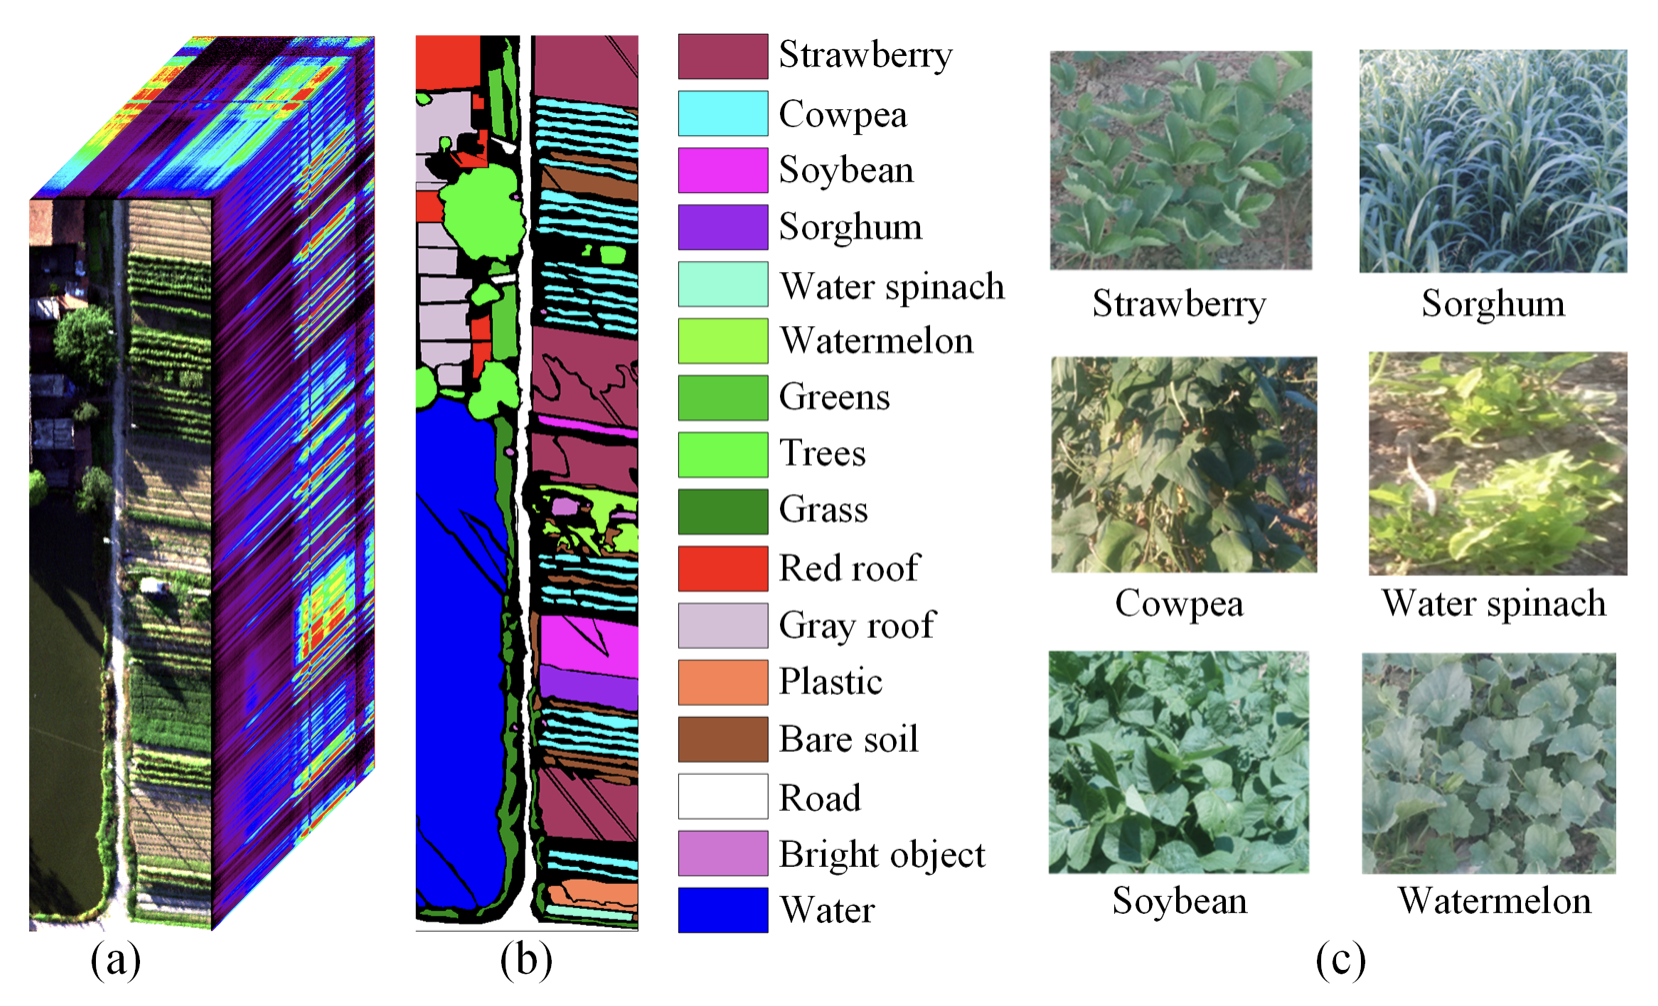
\includegraphics[width=1\linewidth]{WHU-HI_HanChuan274.png}
            \captionsetup{labelformat=simple, labelsep=colon, font=tiny, labelfont={color=gray,bf}}
            \caption{The WHU-Hi-HanChuan dataset was acquired on June 17, 2016, using a UAV-borne hyperspectral imaging sensor. The dataset covers a rural-urban fringe zone and includes seven crop species: strawberry, cowpea, soybean, sorghum, water spinach, watermelon, and greens. The image size is 1217 × 303 pixels, with 274 bands ranging from 400 to 1000 nm. (a) Hyperspectral image cube, (b) ground-truth image, and (c) typical crop photos in the study area. The high dimensionality and complex spectral patterns present challenges for unsupervised clustering and feature extraction.\cite{huWHUHiUAVborneHyperspectral}}
            \label{fig:whu-hi-hanchuan}
            \end{figure}
        \end{column}
        
        % Right column
        \begin{column}{0.62\textwidth}
            \begin{itemize}
                \item \small \textbf{High Dimensionality}: HSI data consists of hundreds of spectral bands, making it computationally challenging to process.
                \item \small \textbf{Complex Patterns}: The spectral information in HSI often includes overlapping and mixed signatures, complicating the clustering process.
                \item \small \textbf{Need for Effective Algorithms}: There is a pressing need for advanced unsupervised clustering algorithms that can efficiently handle the high dimensionality and complexity of HSI data.
            \end{itemize}
        \end{column}
    \end{columns}
\end{frame}

\section{State of the Art (SOTA)}

\subsection{HSI}
\begin{frame}{}
\tiny
\begin{figure}
    \centering
    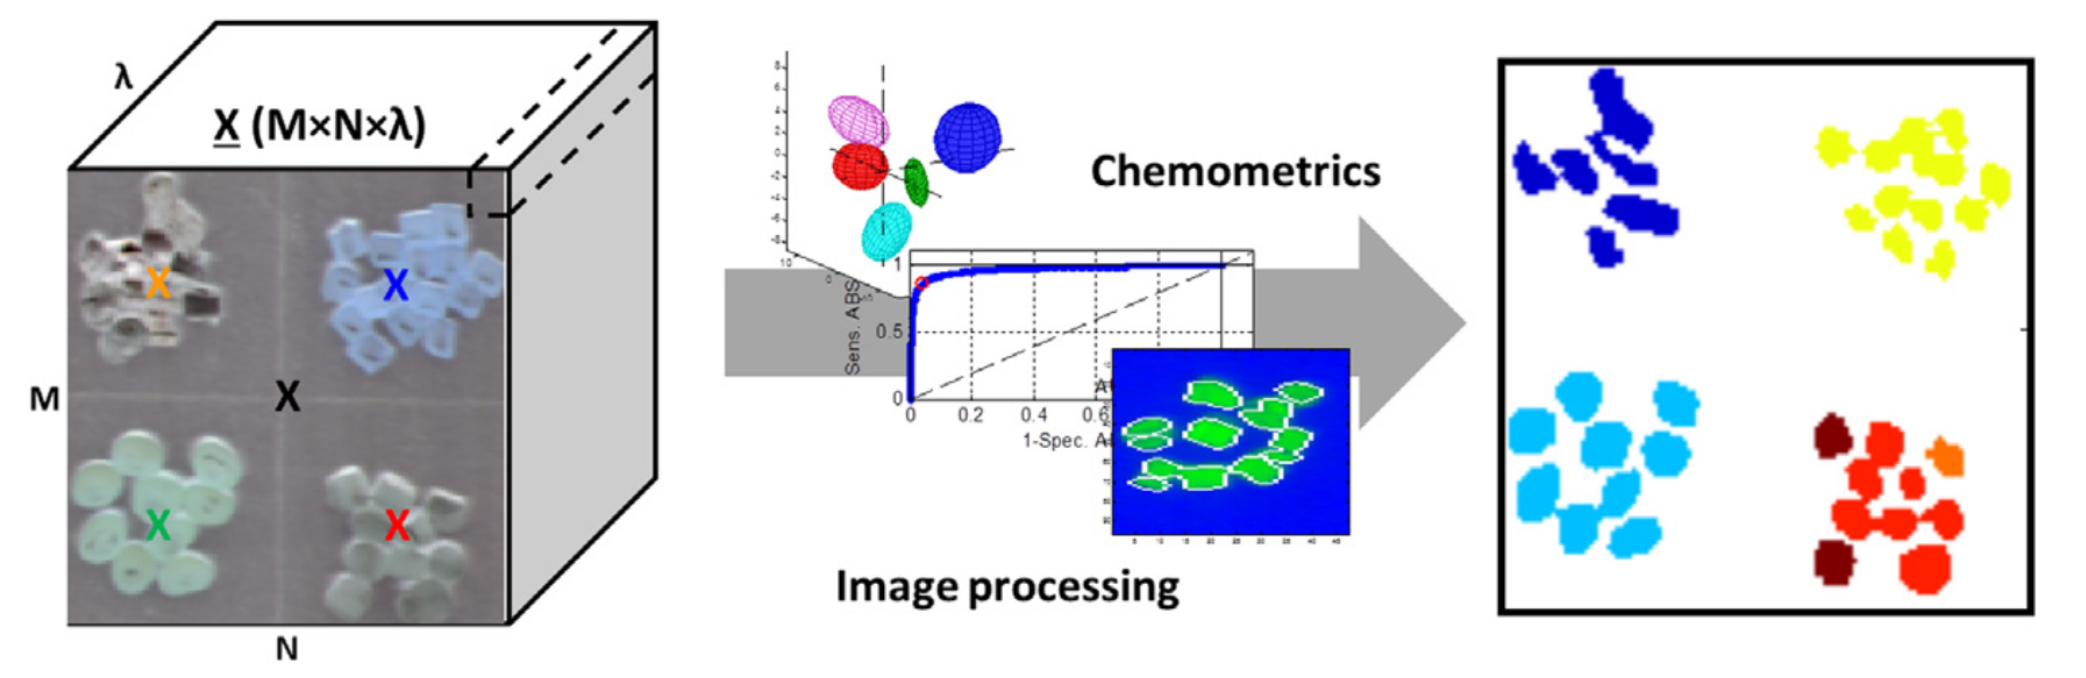
\includegraphics[width=0.62\linewidth]{tutorial_figure.png}
    \captionsetup{labelformat=simple, labelsep=colon, font=tiny, labelfont={color=gray,bf}}
    \caption{\textbf{Graphical Abstract from “Hyperspectral image analysis. A tutorial”} This figure illustrates the hierarchical discrimination of six classes of plastics containing flame retardant using multivariate data analysis and digital image processing methods.\cite{amigoHyperspectralImageAnalysis2015}}
    \label{fig:tutorial_figure}
\end{figure}
\begin{itemize}
    \item Amigo, J.M., Babamoradi, H., Elcoroaristizabal, S. (2015). Hyperspectral Image Analysis: A Tutorial. \textit{Analytica Chimica Acta}, 896, 34-51. \href{https://www.sciencedirect.com/science/article/pii/S0003267015011691}{\color{blue}{DOI: 10.1016/j.aca.2015.09.030}}
    {\color{gray}Provides guidelines and practical tools for analyzing hyperspectral images, focusing on steps like image acquisition, pre-processing, multivariate exploratory analysis, and classification.}
    \begin{itemize} \tiny
    \item \textbf{PLS-DA Model:} Uses Partial Least Squares Discriminant Analysis (PLS-DA) for classification. The model predicts class membership based on the dummy matrix \( \mathbf{D} \), containing binary entries.
    \[
    \hat{\mathbf{Y}} = \mathbf{X} \mathbf{B}
    \]
    Where \( \hat{\mathbf{Y}} \) is the predicted response, \( \mathbf{X} \) is the data matrix, and \( \mathbf{B} \) is the matrix of regression coefficients.
    \item \textbf{Root Mean Square Error (RMSE):} Measures the optimal number of latent variables (LVs).
    \[
    \text{RMSE} = \sqrt{\frac{1}{n} \sum_{i=1}^{n} (\hat{y}_i - y_i)^2}
    \]
    \item \textbf{Classification Metrics:} Includes sensitivity, specificity, and classification error.
    \[
    \text{Sensitivity} = \frac{\text{TP}}{\text{TP} + \text{FN}}, \quad \text{Specificity} = \frac{\text{TN}}{\text{TN} + \text{FP}}, \quad \text{Class Error} = \frac{\text{FP} + \text{FN}}{\text{Total Samples}}
    \]
\end{itemize}

\end{itemize}
\end{frame}
\begin{frame}{}
\tiny
\begin{itemize}

    \item Prasad, S., Bruce, L.M., Chanussot, J. (2015). Introduction to the Issue on Advances in Hyperspectral Data Processing and Analysis. \textit{IEEE Journal of Selected Topics in Applied Earth Observations and Remote Sensing}, 8(6), 2398-2400. \href{https://consensus.app/papers/introduction-issue-advances-hyperspectral-data-prasad/350a2b44cc1a570f86f9e84aca539a5b/?utm_source=chatgpt}{\color{blue}{DOI: 10.1109/JSTARS.2015.2459631}}
    {\color{gray}This special issue covers advances in hyperspectral image-processing research, focusing on novel algorithmic approaches, theoretical insights, and performance limits in image-processing techniques.}
    \begin{itemize} \tiny
    \item \textbf{Parallel Processing:} Implements parallel versions of hyperspectral image processing algorithms to handle large datasets efficiently.
    \[
    S(p) = \frac{T(1)}{T(p)}
    \]
    Where \( S(p) \) is the speedup with \( p \) processors, \( T(1) \) is the execution time with one processor, and \( T(p) \) is the execution time with \( p \) processors.
    \item \textbf{Hierarchical Segmentation:} Segments the image at different levels of detail using region-growing and spectral clustering methods. The convergence criterion for region growing is based on minimizing the within-segment variance.
    \[
    E(S) = \sum_{i=1}^{n} \sum_{x_j \in S_i} (\mathbf{x}_j - \boldsymbol{\mu}_i)^T (\mathbf{x}_j - \boldsymbol{\mu}_i)
    \]
    Where \( S \) is the segmentation, \( S_i \) is the \( i \)-th segment, \( \mathbf{x}_j \) is the \( j \)-th pixel, and \( \boldsymbol{\mu}_i \) is the mean vector of segment \( S_i \).
    \item \textbf{Spectral Mixture Analysis:} Decomposes each pixel's spectrum into a linear combination of endmember spectra.
    \[
    \mathbf{r} = \sum_{i=1}^{n} f_i \mathbf{e}_i
    \]
    Where \( \mathbf{r} \) is the reflectance vector, \( f_i \) are the fractional abundances, and \( \mathbf{e}_i \) are the endmember spectra.
\end{itemize}
    
\end{itemize}
\end{frame}
\begin{frame}{}
\tiny
\begin{itemize}

    \item Plaza, A., Benediktsson, J.A., Boardman, J.W., et al. (2009). Recent Advances in Techniques for Hyperspectral Image Processing. \textit{Remote Sensing of Environment}, 113, S110-S122. \href{https://www.sciencedirect.com/science/article/pii/S0034425709000807}{\color{blue}{DOI: 10.1016/j.rse.2009.01.007}}
    {\color{gray}Provides an overview of recent techniques in hyperspectral image processing, focusing on high-dimensional data handling and the integration of spatial and spectral information.}
    \begin{itemize} \tiny
    \item \textbf{Hierarchical Segmentation:} Segments the image at different levels of detail using region-growing and spectral clustering methods. The convergence criterion for region growing is based on minimizing the within-segment variance.
    \item \textbf{Parallel Processing:} Implements parallel versions of hyperspectral image processing algorithms to handle large datasets efficiently. The speedup is calculated as: \( S(p) = \frac{T(1)}{T(p)} \), where \( T(1) \) is the execution time with one processor and \( T(p) \) is the execution time with \( p \) processors.
    \item \textbf{Kernel Methods:} Kernel-based methods, such as Support Vector Machines (SVM), are used for classification tasks in hyperspectral imaging. The kernel function \( K(x_i, x_j) \) transforms data into a higher-dimensional space to find a hyperplane that maximizes the margin between classes.
    \[
    K(x_i, x_j) = \phi(x_i) \cdot \phi(x_j)
    \]
    \item \textbf{Markov Random Fields (MRF):} MRFs are used to incorporate spatial context in the classification process by modeling the spatial dependencies between neighboring pixels.
    \[
    P(X = x) = \frac{1}{Z} \exp\left( - \sum_{c \in C} \psi_c(x_c) \right)
    \]
    Where \( Z \) is the partition function, \( \psi_c \) are the potential functions over cliques \( c \).
    \item \textbf{Spectral Mixture Analysis:} This technique decomposes each pixel's spectrum into a linear combination of endmember spectra.
    \[
    \mathbf{r} = \sum_{i=1}^{n} f_i \mathbf{e}_i
    \]
    Where \( \mathbf{r} \) is the reflectance vector, \( f_i \) are the fractional abundances, and \( \mathbf{e}_i \) are the endmember spectra.
\end{itemize}

\end{itemize}
\end{frame}
\begin{frame}{}
\tiny
\begin{itemize}

   \item Khan, M.J., Khan, H.S., Yousaf, A., et al. (2018). Modern Trends in Hyperspectral Image Analysis: A Review. \textit{IEEE Geoscience and Remote Sensing Magazine}, 6(3), 21-28. \href{https://ieeexplore.ieee.org/document/8454602}{\color{blue}{DOI: 10.1109/MST.2018.2806959}}
    {\color{gray}Reviews modern trends in hyperspectral image analysis, including applications in food quality assessment, medical diagnosis, and forensic science.}
    \begin{itemize} \tiny
    \item \textbf{Data Fusion:} Combines data from multiple sources to improve accuracy and reliability.
    \[
    \mathbf{D}_{fused} = f(\mathbf{D}_1, \mathbf{D}_2, \ldots, \mathbf{D}_n)
    \]
    Where \( \mathbf{D}_{fused} \) is the fused dataset, and \( f \) is the fusion function.
    \item \textbf{Anomaly Detection:} Identifies outliers in hyperspectral images.
    \[
    \text{Anomaly Score} = \frac{(\mathbf{x} - \boldsymbol{\mu})^T \boldsymbol{\Sigma}^{-1} (\mathbf{x} - \boldsymbol{\mu})}{\sqrt{2 \pi |\boldsymbol{\Sigma}|}}
    \]
    Where \( \mathbf{x} \) is the pixel vector, \( \boldsymbol{\mu} \) is the mean vector, and \( \boldsymbol{\Sigma} \) is the covariance matrix.
    \item \textbf{Hyperspectral Unmixing:} Decomposes mixed pixels into their constituent endmember spectra and corresponding abundances.
    \[
    \mathbf{R} = \mathbf{EA} + \mathbf{N}
    \]
    Where \( \mathbf{R} \) is the reflectance matrix, \( \mathbf{E} \) is the endmember matrix, \( \mathbf{A} \) is the abundance matrix, and \( \mathbf{N} \) is the noise matrix.
\end{itemize}

\end{itemize}
\end{frame}
\begin{frame}{}
\tiny
\begin{itemize}

    \item Vidal, M., Amigo, J.M. (2012). Pre-processing of Hyperspectral Images: Essential Steps Before Image Analysis. \textit{Chemometrics and Intelligent Laboratory Systems}, 117, 138-148. \href{https://www.sciencedirect.com/science/article/pii/S0169743912001503}{\color{blue}{DOI: 10.1016/j.chemolab.2012.05.009}}
    {\color{gray}Discusses the necessary pre-processing steps for hyperspectral images, such as background removal and image compression, to enhance data analysis.}
    \begin{itemize} \tiny
    \item \textbf{Image Compression:} Uses methods like PCA (Principal Component Analysis) for data compression.
    \[
    \mathbf{X} \approx \mathbf{T} \mathbf{P}^T
    \]
    Where \( \mathbf{X} \) is the original data matrix, \( \mathbf{T} \) are the scores, and \( \mathbf{P} \) are the loadings.
    \item \textbf{Wavelet Transform:} Applies wavelet transform for noise reduction and data compression.
    \[
    f(t) = \sum_{k=1}^{n} c_k \psi_k(t)
    \]
    Where \( c_k \) are wavelet coefficients and \( \psi_k(t) \) are wavelet functions.
    \item \textbf{Background Removal:} Utilizes thresholding based on PCA scores to distinguish sample from background.
    \[
    \text{Threshold} = \text{mean}(\mathbf{T}) + k \cdot \text{std}(\mathbf{T})
    \]
\end{itemize}
    
\end{itemize}
\end{frame}
\begin{frame}{}
\tiny
\begin{itemize}

    \item Camps-Valls, G., Bruzzone, L. (2005). Kernel-based Methods for Hyperspectral Image Classification. \textit{IEEE Transactions on Geoscience and Remote Sensing}, 43(6), 1351-1362. \href{https://ieeexplore.ieee.org/document/1421797}{\color{blue}{DOI: 10.1109/TGRS.2005.846154}}
    {\color{gray}Presents the framework of kernel-based methods for hyperspectral image classification, comparing different approaches and analyzing their properties in the hyperspectral domain.}
    \begin{itemize} \tiny
    \item \textbf{Support Vector Machines (SVM):} Uses a decision function for classification.
    \[
    f(x) = \sum_{i=1}^{n} \alpha_i y_i K(x_i, x) + b
    \]
    Where \( \alpha_i \) are the Lagrange multipliers, \( y_i \) are the class labels, \( K \) is the kernel function, and \( b \) is the bias term.
    \item \textbf{Kernel Fisher Discriminant (KFD):} Projects data onto a direction that maximizes class separability.
    \[
    J(w) = \frac{w^T S_B w}{w^T S_W w}
    \]
    Where \( S_B \) is the between-class scatter matrix, and \( S_W \) is the within-class scatter matrix.
    \item \textbf{Least Squares SVM (LS-SVM):} Solves a set of linear equations for optimization.
    \[
    \min_w \frac{1}{2} w^T w + \frac{\gamma}{2} \sum_{i=1}^{n} e_i^2 \quad \text{subject to} \quad y_i (w^T \phi(x_i) + b) = 1 - e_i
    \]
    Where \( \gamma \) is the regularization parameter, and \( e_i \) are the error variables.
\end{itemize}
    
\end{itemize}
\end{frame}
\begin{frame}{}
\tiny
\begin{itemize}

    \item Selci, S. (2019). The Future of Hyperspectral Imaging. \textit{Journal of Biomedical Optics}, 24(6), 1-11. \href{https://www.spiedigitallibrary.org/journals/journal-of-biomedical-optics/volume-24/issue-6/061207/Medical-hyperspectral-imaging-a-review/10.1117/1.JBO.24.6.061207.full}{\color{blue}{DOI: 10.1117/1.JBO.24.6.061207}}
    {\color{gray}Explores future trends in hyperspectral imaging, covering specific current research, updates on methodological tools, and emerging applications.}
    \begin{itemize} \tiny
    \item \textbf{Spectral Data Fusion:} Combines spectral data from different sources using methods like partial least squares regression (PLSR).
    \[
    \mathbf{Y} = \mathbf{X}\mathbf{B} + \mathbf{E}
    \]
    where \(\mathbf{Y}\) is the dependent variable matrix, \(\mathbf{X}\) is the independent variable matrix, \(\mathbf{B}\) is the regression coefficient matrix, and \(\mathbf{E}\) is the error matrix.
    \item \textbf{Principal Component Analysis (PCA):} Used for dimensionality reduction in hyperspectral data.
    \[
    \mathbf{X} = \mathbf{TP}^T + \mathbf{E}
    \]
    where \(\mathbf{X}\) is the data matrix, \(\mathbf{T}\) are the scores, \(\mathbf{P}\) are the loadings, and \(\mathbf{E}\) is the residual matrix.
    \item \textbf{Classification Techniques:} Methods like k-nearest neighbors (KNN) and support vector machines (SVM) are used for classification tasks.
    \begin{itemize} \tiny
        \item \textbf{KNN:}
        \[
        d(x, y) = \sqrt{\sum_{i=1}^{n} (x_i - y_i)^2}
        \]
        where \(d(x, y)\) is the distance between points \(x\) and \(y\).
        \item \textbf{SVM:}
        \[
        f(x) = \sum_{i=1}^{n} \alpha_i y_i K(x_i, x) + b
        \]
        where \(\alpha_i\) are the Lagrange multipliers, \(y_i\) are the class labels, \(K\) is the kernel function, and \(b\) is the bias term.
    \end{itemize}
    \item \textbf{Image Registration:} Aligns hyperspectral images taken at different times or from different sensors.
    \[
    \text{MI}(A, B) = \sum_{a \in A} \sum_{b \in B} p(a, b) \log \frac{p(a, b)}{p(a)p(b)}
    \]
    where \(\text{MI}(A, B)\) is the mutual information between images \(A\) and \(B\).
\end{itemize}

\end{itemize}
\end{frame}
\begin{frame}
\tiny
\begin{itemize}

    \item Lu, G., Fei, B. (2014). Medical Hyperspectral Imaging: A Review. \textit{Journal of Biomedical Optics}, 19(1), 010901. \href{https://www.spiedigitallibrary.org/journals/journal-of-biomedical-optics/volume-19/issue-01/010901/Medical-hyperspectral-imaging-a-review/10.1117/1.JBO.19.1.010901.full}{\color{blue}{DOI: 10.1117/1.JBO.19.1.010901}}
    {\color{gray}Reviews the applications of hyperspectral imaging in medical fields, particularly in disease diagnosis and image-guided surgery.}
    \begin{itemize} \tiny
    \item \textbf{Tissue Optics:}
    \begin{itemize} \tiny
        \item \textbf{Beer-Lambert Law:}
        \[
        A(\lambda) = \log_{10}\left(\frac{I_0(\lambda)}{I(\lambda)}\right) = \epsilon(\lambda) c L
        \]
        where \(A(\lambda)\) is absorbance, \(I_0(\lambda)\) is the incident light intensity, \(I(\lambda)\) is the transmitted light intensity, \(\epsilon(\lambda)\) is the molar absorptivity, \(c\) is the concentration, and \(L\) is the path length.
        \item \textbf{Light Scattering:} Described using Mie and Rayleigh scattering models.
        \[
        \text{Scattering Coefficient} = \frac{24\pi^3 r^6}{\lambda^4} \left(\frac{n^2-1}{n^2+2}\right)^2
        \]
        where \(r\) is the particle radius, \(\lambda\) is the wavelength, and \(n\) is the refractive index.
    \end{itemize}
    \item \textbf{Fluorescence:} Fluorescence intensity \(I_f\) is proportional to the concentration of fluorophores \(c_f\) and the quantum yield \(\Phi\):
    \[
    I_f \propto c_f \Phi I_0
    \]
    where \(I_0\) is the incident light intensity.
    \item \textbf{Principal Component Analysis (PCA):} Dimensionality reduction method.
    \[
    \mathbf{X} = \mathbf{TP}^T + \mathbf{E}
    \]
    where \(\mathbf{X}\) is the data matrix, \(\mathbf{T}\) are the scores, \(\mathbf{P}\) are the loadings, and \(\mathbf{E}\) is the residual matrix.
    \item \textbf{Support Vector Machines (SVM):} Classification method.
    \[
    f(x) = \sum_{i=1}^{n} \alpha_i y_i K(x_i, x) + b
    \]
    where \(\alpha_i\) are the Lagrange multipliers, \(y_i\) are the class labels, \(K\) is the kernel function, and \(b\) is the bias term.
    \item \textbf{Spectral Angle Mapper (SAM):} Measures the spectral similarity between two spectra.
    \[
    \theta = \cos^{-1} \left(\frac{\mathbf{t} \cdot \mathbf{r}}{\|\mathbf{t}\| \|\mathbf{r}\|}\right)
    \]
    where \(\mathbf{t}\) is the target spectrum, and \(\mathbf{r}\) is the reference spectrum.
\end{itemize}

\end{itemize}
\end{frame}
\begin{frame}
\tiny
\begin{itemize}

    \item Kwon, H., Nasrabadi, N.M., Bandos, T.V., et al. (2013). Algorithms for Multispectral and Hyperspectral Image Analysis. \textit{Journal of Electrical and Computer Engineering}, 2013, Article ID 917203. \href{https://www.hindawi.com/journals/jece/2013/917203/}{\color{blue}{DOI: 10.1155/2013/917203}}
    {\color{gray}Focuses on advances in algorithms and technologies for multispectral and hyperspectral imagery, addressing critical issues such as anomaly detection and target classification.}
    
    \item Grahn, H., Geladi, P. (2007). Techniques and Applications of Hyperspectral Image Analysis. \textit{Techniques and Applications of Hyperspectral Image Analysis}, John Wiley \& Sons. \href{https://books.google.com/books?id=2ifVDwAAQBAJ}{\color{blue}{DOI: 10.1002/9780470010861}}

    {\color{gray}Provides a comprehensive overview of various techniques and applications in hyperspectral image analysis, covering principles of multivariate image analysis, clustering, classification, and calibration standards.}
\end{itemize}
\end{frame}













\begin{frame}{}
\tiny
\begin{figure}
    \centering
            \centering
            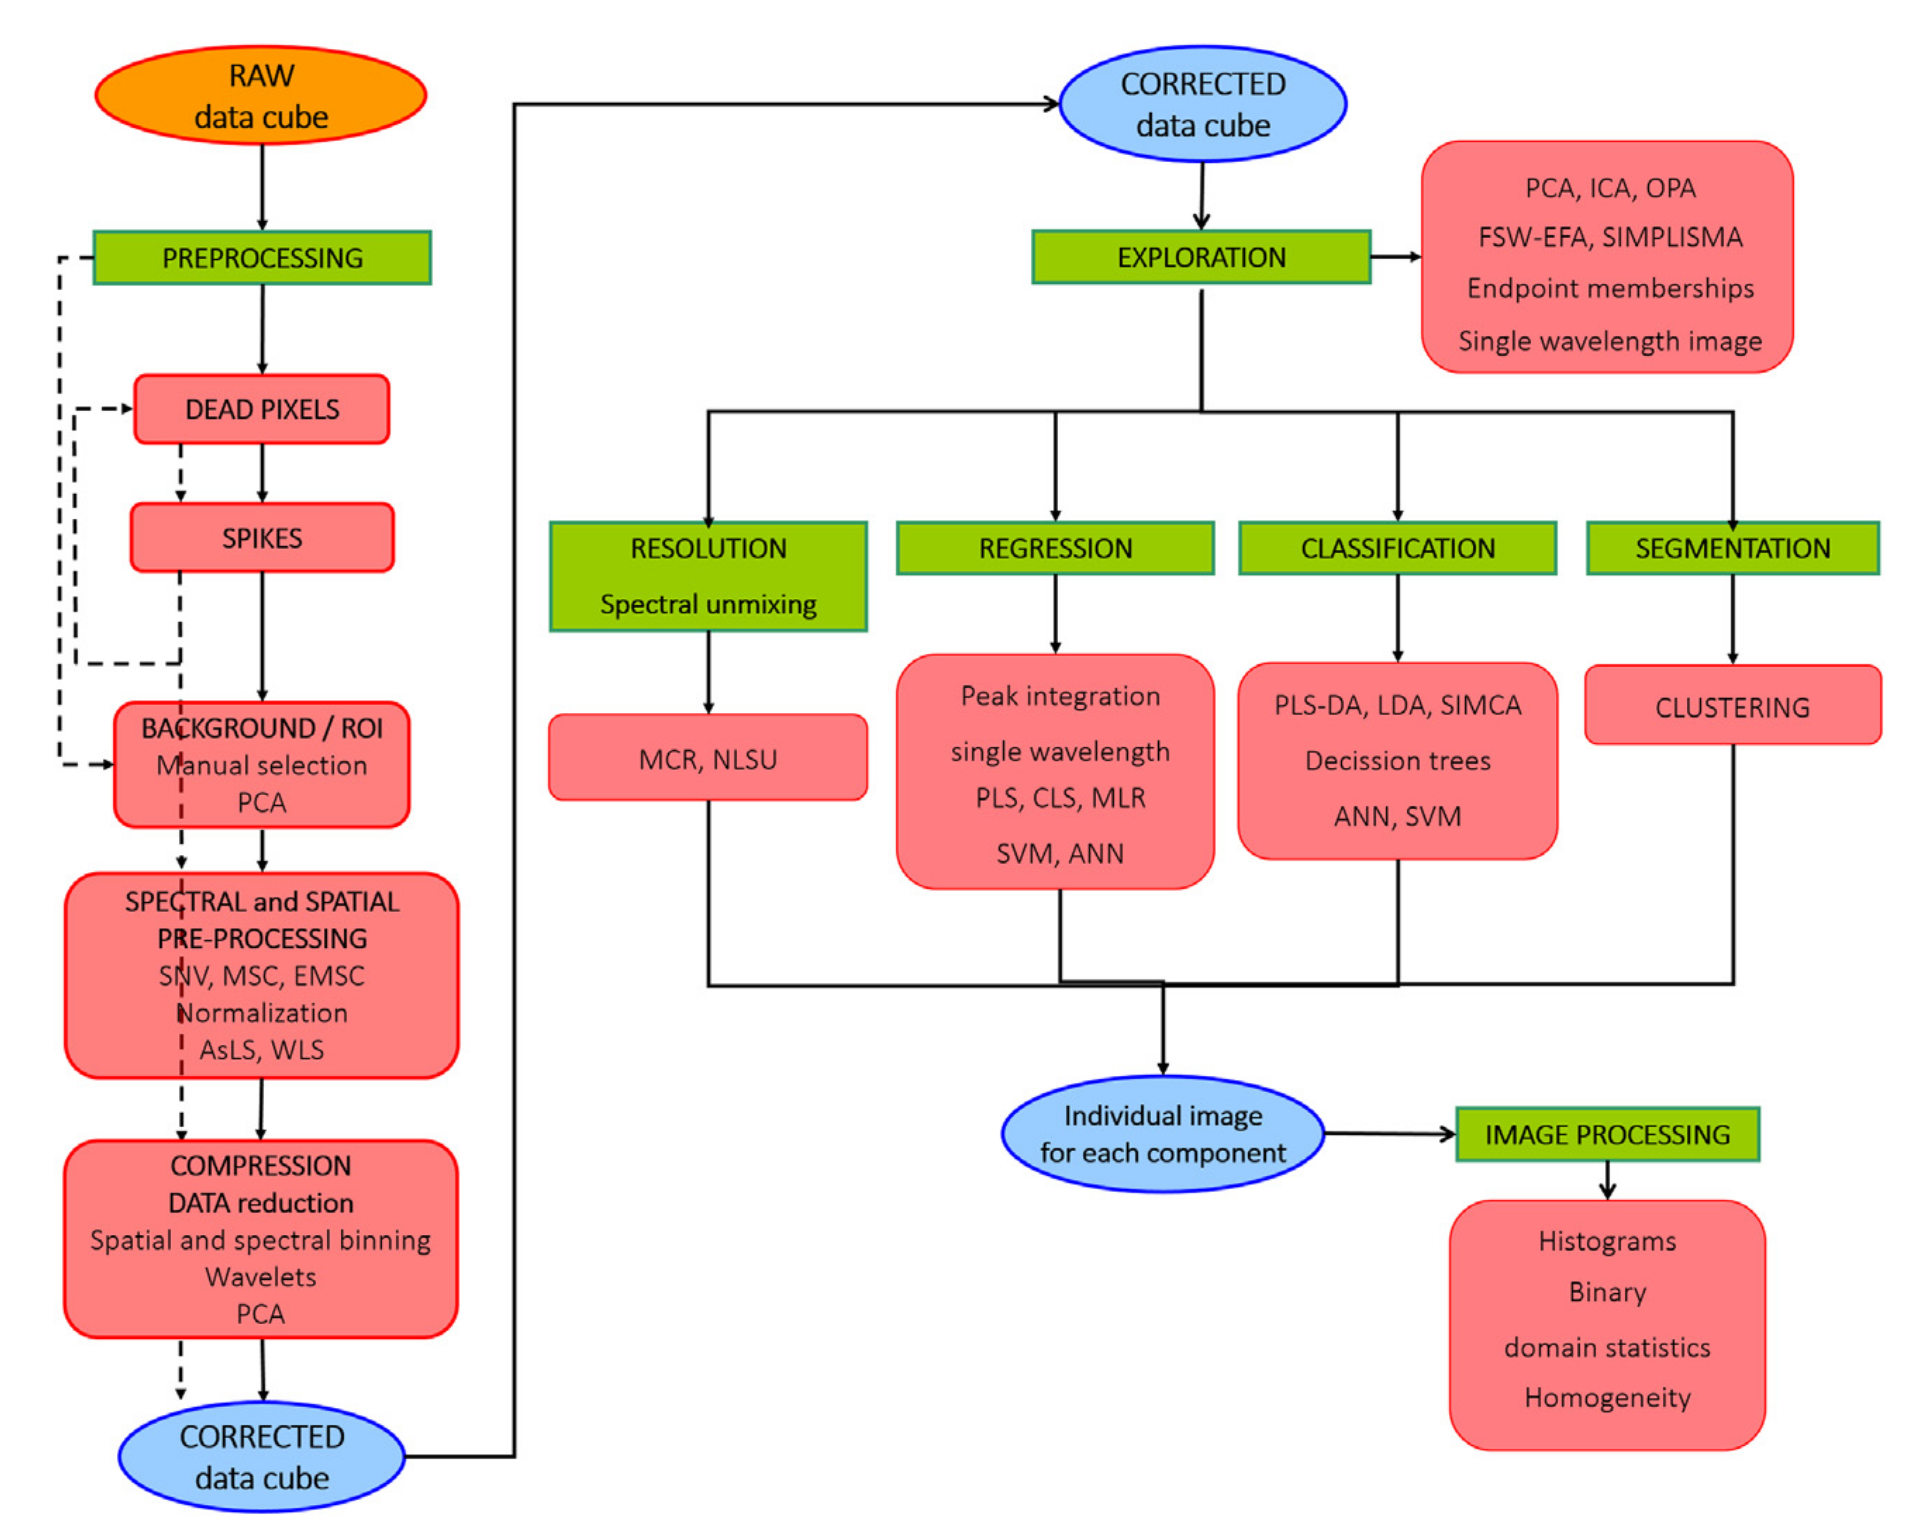
\includegraphics[width=0.62\linewidth]{amigo_chart.png}
            \captionsetup{labelformat=simple, labelsep=colon, font=tiny, labelfont={color=gray,bf}}
            \caption{\textbf{Comprehensive Flowchart of Hyperspectral and Multispectral Image Analysis} This flowchart outlines the complete process of hyperspectral and multispectral image analysis. It begins with preprocessing the raw data cube, addressing issues like dead pixels and spikes, and includes steps such as spectral and spatial preprocessing, data compression, and correction. The corrected data cube is then explored using techniques like PCA, ICA, and SIMPLISMA. The analysis continues with resolution (spectral unmixing), regression (peak integration, PLS, SVM), classification (PLS-DA, LDA, ANN), and segmentation (clustering). The final stage involves image processing for histogram analysis, binary domain statistics, and homogeneity. (Adapted from Amigo et al., 2015)\cite{amigoHyperspectralMultispectralImaging2019}}
    \label{fig:amigo_chart}
\end{figure}

\end{frame}
\begin{frame}
\tiny
\begin{itemize}

\item Amigo, J.M. (2019). Hyperspectral and Multispectral Imaging: Setting the Scene. \textit{Hyperspectral Imaging}. Elsevier. \href{https://doi.org/10.1016/B978-0-444-63977-6.00001-8}{\color{blue}{DOI: 10.1016/B978-0-444-63977-6.00001-8}}
{\color{gray}Discusses the basic concepts of hyperspectral and multispectral imaging, including spatial resolution, types of images, data mining, and chemometrics.}
\begin{itemize} \tiny
    \item \textbf{Spatial Resolution:}
    \[
    \text{Resolution} = \frac{\text{Image Size}}{\text{Pixel Size}}
    \]
    \item \textbf{Single Channel Images:}
    \[
    I(x, y)
    \]
    \item \textbf{Color-Space Images:}
    \[
    \text{RGB} = (R, G, B)
    \]
    \item \textbf{Multiband Images:}
    \[
    \{I_{\lambda_1}, I_{\lambda_2}, \ldots, I_{\lambda_n}\}
    \]
    \item \textbf{Hyperspectral Images:}
    \[
    \{I(\lambda_1), I(\lambda_2), \ldots, I(\lambda_n)\}
    \]
    \item \textbf{Chemometrics:}
    \[
    \text{Hypercube} = (X \times Y \times \lambda)
    \]
    \item \textbf{Preprocessing:}
    \[
    I_{\text{normalized}} = \frac{I_{\text{raw}} - I_{\text{dark}}}{I_{\text{white}} - I_{\text{dark}}}
    \]
    \item \textbf{Pattern Recognition/Exploration:}
    \[
    \mathbf{X} = \mathbf{T} \mathbf{P}^T + \mathbf{E}
    \]
    \item \textbf{Segmentation:}
    \[
    \min \sum_{i=1}^{k} \sum_{x_j \in C_i} \|x_j - \mu_i\|^2
    \]
    \item \textbf{Curve Resolution Methods/Spectral Unmixing:}
    \[
    \mathbf{D} = \mathbf{C} \mathbf{S} + \mathbf{E}
    \]
    \item \textbf{Regression and Classification:}
    \[
    \mathbf{Y} = \mathbf{X} \mathbf{B}
    \]
\end{itemize}

\end{itemize}
\end{frame}
\begin{frame}
\tiny
\begin{itemize}

    \item Lu, B., Dao, P.D., Liu, J., et al. (2020). Recent Advances of Hyperspectral Imaging Technology and Applications in Agriculture. \textit{Remote Sensing}, 12(15), 2659. \href{https://www.mdpi.com/2072-4292/12/15/2659}{\color{blue}{DOI: 10.3390/rs12152659}}
    {\color{gray}Reviews recent advancements in hyperspectral imaging technology and its applications in agriculture, discussing mini-sized and low-cost airborne hyperspectral sensors.}
    \begin{itemize} \tiny
    \item \textbf{Support Vector Machines (SVM):} SVM classifiers are used with kernel functions to handle the high-dimensional hyperspectral data. The classification function is given by: \[ f(x) = \sum_{i=1}^{n} \alpha_i K(x, x_i) + b \], where \( K \) is the kernel function.
    \item \textbf{Markov Random Fields (MRF):} MRF models the spatial dependencies between pixels. The energy function to be minimized is: \[ E(x) = \sum_{i} U(x_i) + \sum_{i,j} V(x_i, x_j) \], where \( U \) is the unary potential and \( V \) is the pairwise potential.
    \item \textbf{Morphological Processing:} Uses mathematical morphology for feature extraction. The extended morphological profiles (EMP) are constructed by applying morphological operators to hyperspectral data.
\end{itemize}

\end{itemize}
\end{frame}
\begin{frame}
\tiny
\begin{itemize}

\item Manolakis, D., Shaw, G. (2002). Detection Algorithms for Hyperspectral Imaging Applications. \textit{IEEE Signal Processing Magazine}, 19(1), 29-43. \href{https://ieeexplore.ieee.org/document/974635}{\color{blue}{DOI: 10.1109/79.974635}}
    {\color{gray}Provides a comprehensive review of detection algorithms used in hyperspectral imaging applications, covering both conventional and contemporary methods.
    \begin{itemize} \tiny
    \item \textbf{Geometric Approach:} The spectrum vector \( x \) is modeled as a linear combination of basis vectors: \[ x = \sum_{k=1}^{M} a_k s_k \] where \( a_k \) are coefficients and \( s_k \) are basis vectors.
    \item \textbf{Statistical Approach:} Hyperspectral data is modeled using multivariate normal distributions. The likelihood ratio test (LRT) is used for detection: \[ y = (\mu_b - \mu_t)^T \Sigma^{-1} x \], where \( \mu_b \) and \( \mu_t \) are the mean vectors of the background and target, and \( \Sigma \) is the covariance matrix.
    \item \textbf{Matched Filter (MF):} Derived by maximizing the signal-to-noise ratio (SNR), resulting in the filter: \[\ c_{MF} = \Sigma^{-1} (\mu_t - \mu_b) \].
    \item \textbf{Adaptive Coherence Estimator (ACE):} Uses the whitening transformation to express the detector as: \[ D_{ACE}(x) = \cos^2 (\theta) \], where \( \theta \) is the angle between the test pixel and the target subspace in the whitened space.
    \end{itemize}}

\end{itemize}
\end{frame}
\begin{frame}{}
\tiny
\begin{itemize}
    
    \item Calin, M.A., Parasca, S.V., Savastru, D., et al. (2014). Hyperspectral Imaging in the Medical Field: Present and Future. \textit{Applied Spectroscopy Reviews}, 49(6), 435-447. \href{https://www.tandfonline.com/doi/abs/10.1080/05704928.2014.881309}{\color{blue}{DOI: 10.1080/05704928.2014.881309}}
    {\color{gray}Reviews the current state and future prospects of hyperspectral imaging in medical applications, particularly in disease diagnosis and therapeutic monitoring.}
    \begin{itemize} \tiny
    \item \textbf{Cancer Detection:} Hyperspectral imaging (HSI) is used to detect various types of cancer. The sensitivity and specificity are calculated using the confusion matrix. For example, for gastric cancer: sensitivity = 93\%, specificity = 91\%.
    \item \textbf{Diabetic Foot Ulcers:} HSI measures tissue oxygenation (oxyhemoglobin and deoxyhemoglobin) to predict ulcer healing. The healing prediction index is derived using logistic regression: \[ P(\text{healing}) = \frac{1}{1 + e^{-(a + b_1 \cdot \text{oxy} + b_2 \cdot \text{deoxy})}} \].
    \item \textbf{Tissue Oxygenation:} Uses the modified Beer-Lambert law to produce maps of oxyhemoglobin and deoxyhemoglobin concentrations: \[ A(\lambda) = \log_{10}\left(\frac{I_0(\lambda)}{I(\lambda)}\right) = \epsilon(\lambda) c L \], where \( A(\lambda) \) is absorbance, \( \epsilon(\lambda) \) is the molar absorptivity, \( c \) is the concentration, and \( L \) is the path length.
\end{itemize}

\end{itemize}
\end{frame}
\begin{frame}{}
\tiny
\begin{itemize}

    \item Barnes, M., Pan, Z., Zhang, S. (2015). Systems and Methods for Hyperspectral Imaging. \textit{US Patent 9,117,133}. \href{https://patents.google.com/patent/US9117133B2/en}{\color{blue}{DOI: 10.1109/TGRS.2015.2421060}}
    {\color{gray}Describes various systems and methods for hyperspectral imaging, emphasizing the technological advancements and applications in different fields.}
    \begin{itemize} \tiny
    \item \textbf{Neural Networks:} Uses neural networks for classification.
    \[
    J = E + \lambda \|W\|^2
    \]
    Where \( J \) is the new criterion, \( E \) is the training error, \( \lambda \) is the regularization parameter, and \( \|W\| \) is the weight norm.
    \item \textbf{Pruning Algorithms:} Uses Optimal Brain Damage (OBD) and Optimal Brain Surgeon (OBS) for weight elimination.
    \[
    \Delta E \approx \frac{1}{2} \Delta W^T H \Delta W
    \]
    Where \( H \) is the Hessian matrix.
    \item \textbf{Similarity Metrics:} Calculates similarity metrics for spectral signatures.
    \[
    \text{Similarity Metric} = \frac{\sum (x_i - \mu_x)(y_i - \mu_y)}{\sqrt{\sum (x_i - \mu_x)^2 \sum (y_i - \mu_y)^2}}
    \]
\end{itemize}

\end{itemize}
\end{frame}
\begin{frame}{}
\tiny
\begin{itemize}

    \item Fei, B. (2019). Hyperspectral Imaging in Medical Applications. In Q. Liu \& Y. Li (Eds.), \textit{Hyperspectral Imaging} (pp. 523-550). Elsevier. \href{https://doi.org/10.1016/B978-0-444-63977-6.00021-3}{\color{blue}{DOI: 10.1016/B978-0-444-63977-6.00021-3}}
    {\color{gray}Explores the applications of hyperspectral imaging in the medical field, emphasizing its potential for noninvasive disease diagnosis and surgical guidance.}
    \begin{itemize} \tiny
    \item \textbf{Oxyhemoglobin and Deoxyhemoglobin Measurements:} Uses the Beer-Lambert law for tissue oxygenation.
    \[
    A(\lambda) = \epsilon_{\text{HbO}_2}(\lambda) c_{\text{HbO}_2} + \epsilon_{\text{Hb}}(\lambda) c_{\text{Hb}}
    \]
    Where \( A(\lambda) \) is the absorbance, \( \epsilon \) are the molar absorptivity coefficients, and \( c \) are the concentrations.
    \item \textbf{Principal Component Analysis (PCA):} Reduces dimensionality in hyperspectral data.
    \[
    \mathbf{X} = \mathbf{TP}^T + \mathbf{E}
    \]
    Where \( \mathbf{X} \) is the data matrix, \( \mathbf{T} \) are the scores, \( \mathbf{P} \) are the loadings, and \( \mathbf{E} \) is the residual matrix.
\end{itemize}

\end{itemize}
\end{frame}
\begin{frame}{}
\tiny
\begin{itemize}

    \item Landgrebe, D. (2002). Hyperspectral Image Data Analysis. \textit{IEEE Signal Processing Magazine}, 18(1), 17-28. \href{https://ieeexplore.ieee.org/document/1352410}{\color{blue}{DOI: 10.1109/79.939829}}
    {\color{gray}Discusses the evolution and techniques of hyperspectral image data analysis, highlighting the multispectral approach and its applications in remote sensing.}
    \begin{itemize} \tiny
    \item \textbf{Class Density Functions:} Uses discriminant functions for classification. For two classes with means \( \mu_f \) and \( \mu_g \) and covariance matrices \( \Sigma_f \) and \( \Sigma_g \), the quadratic classifier is: \[ g_i(x) = -\frac{1}{2} (x - \mu_i)^T \Sigma_i^{-1} (x - \mu_i) - \frac{1}{2} \log |\Sigma_i| \].
    \item \textbf{Linear Discriminant Analysis (LDA):} Maximizes the ratio of between-class variance to within-class variance: \[ J(w) = \frac{w^T S_b w}{w^T S_w w} \], where \( S_b \) and \( S_w \) are the between-class and within-class scatter matrices.
\end{itemize}

\end{itemize}
\end{frame}
\begin{frame}{}
\tiny
\begin{itemize}

    \item Kerekes, J.P., Baum, J.E. (2003). Hyperspectral Imaging System Modeling. \textit{Lincoln Laboratory Journal}, 14(1), 3-32. \href{https://apps.dtic.mil/sti/citations/ADA415477}{\color{blue}{DOI: 10.1109/TGRS.2003.814658}}
    {\color{gray}Discusses the modeling of hyperspectral imaging systems, including sensor design, calibration, and performance evaluation.}

    \item Manolakis, D., Marden, D., Kerekes, J.P. (2001). Statistics of Hyperspectral Imaging Data. \textit{SPIE Optical Engineering}, 40(8), 2082-2094. \href{https://www.spiedigitallibrary.org/journals/optical-engineering/volume-40/issue-8/2082/Statistics-of-hyperspectral-imaging-data/10.1117/1.1394690.full}{\color{blue}{DOI: 10.1117/1.1394690}}
    {\color{gray}Analyzes the statistical properties of hyperspectral imaging data, providing insights into data characterization and noise reduction techniques.}
    
    \item ElMasry, G., Sun, D.W. (2010). Principles of Hyperspectral Imaging Technology. \textit{Hyperspectral Imaging for Food Quality Analysis and Control}, 3-43. \href{https://www.elsevier.com/books/hyperspectral-imaging-for-food-quality-analysis-and-control/sun/978-0-12-374753-2}{\color{blue}{DOI: 10.1016/B978-0-12-374753-2.00001-8}}
    {\color{gray}Discusses the principles of hyperspectral imaging technology, focusing on its application in food quality analysis.}
\end{itemize}
\end{frame}














\subsection{Unsupervised Clustering in HSI}
\begin{frame}{}
\tiny
\begin{figure}
    \centering
            \centering
            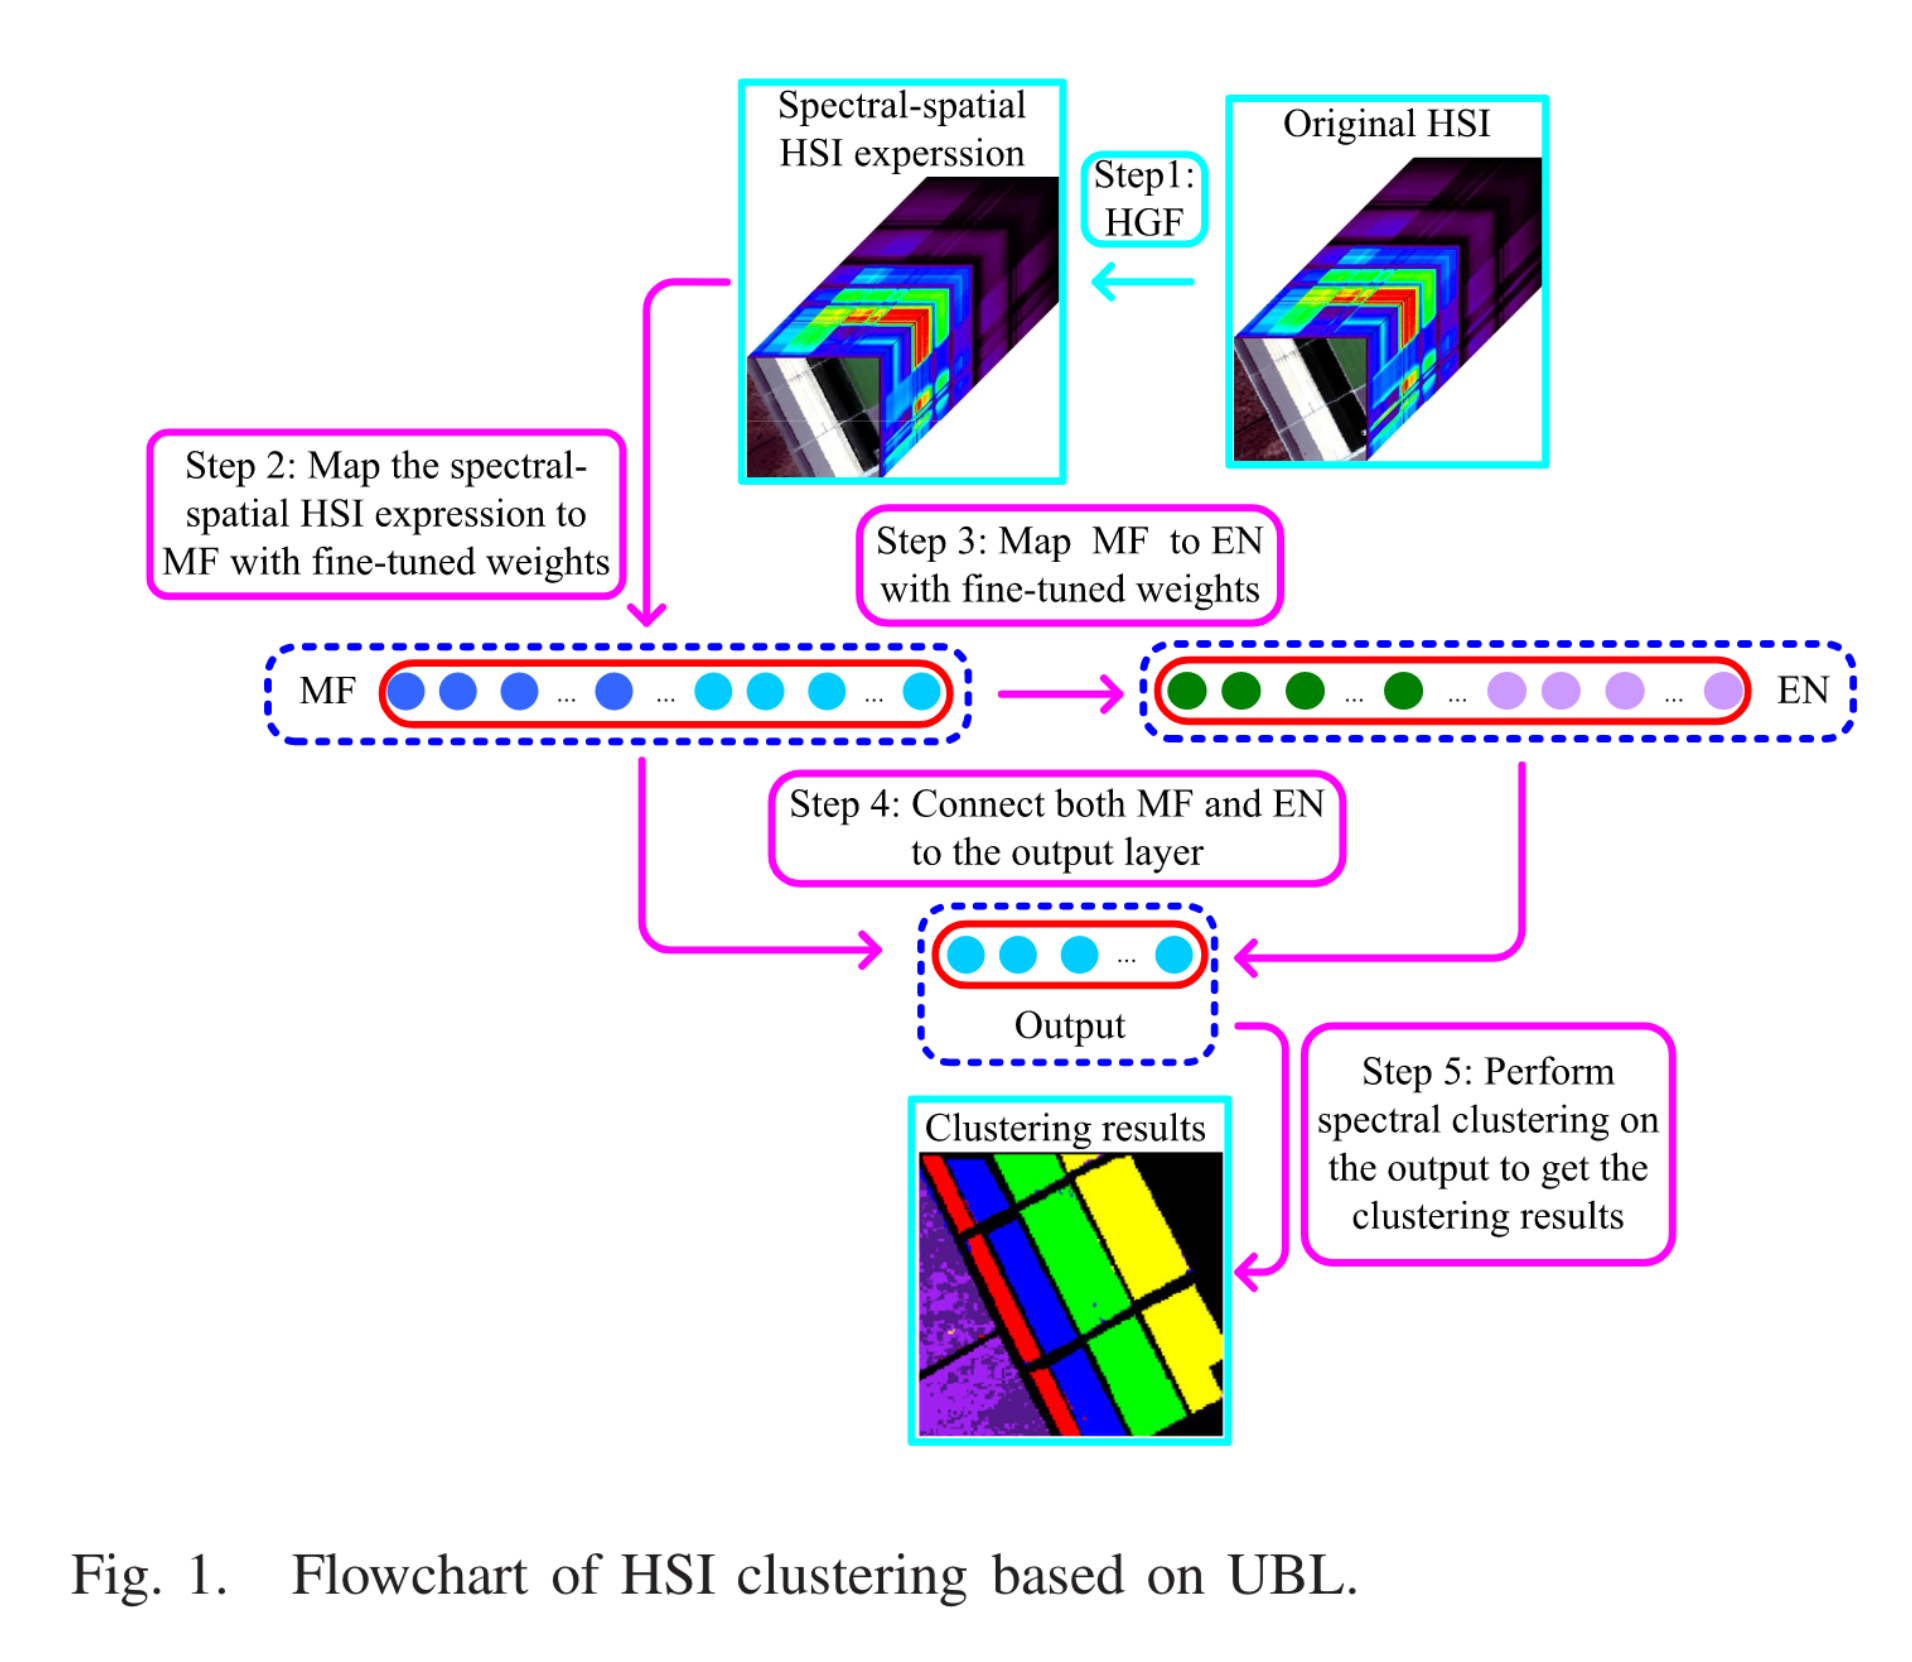
\includegraphics[width=0.62\linewidth]{kong_chat.png}
            \captionsetup{labelformat=simple, labelsep=colon, font=tiny, labelfont={color=gray,bf}}
            \caption{\textbf{Flowchart of HSI Clustering Based on Unsupervised Broad Learning (UBL)} This flowchart illustrates the process of hyperspectral image (HSI) clustering using UBL. Step 1 involves extracting the spectral-spatial HSI expression from the original HSI using hierarchical Gaussian filtering (HGF). In Step 2, the spectral-spatial HSI expression is mapped to the middle feature (MF) layer with fine-tuned weights. Step 3 maps the MF layer to the end feature (EN) layer with fine-tuned weights. Step 4 connects both MF and EN layers to the output layer. Finally, Step 5 performs spectral clustering on the output to obtain the clustering results.\cite{kongHyperspectralImageClustering2019}}
    \label{fig:kong_chart}
\end{figure}
\end{frame}
\begin{frame}
\tiny
\begin{itemize}
\item Kong, Y., Cheng, Y., Chen, C. L. P., \& Wang, X. (2019). Hyperspectral Image Clustering Based on Unsupervised Broad Learning. \textit{IEEE Geoscience and Remote Sensing Letters}, 16(11), 1741-1745. \href{https://doi.org/10.1109/LGRS.2019.2907598}{\color{blue}{DOI: 10.1109/LGRS.2019.2907598}}
{\color{gray}Introduces a novel unsupervised broad learning (UBL) method for hyperspectral image clustering, leveraging graph-regularized sparse autoencoders to preserve intrinsic manifold structure.}
\begin{itemize} \tiny
    \item \textbf{Graph-regularized Sparse Autoencoder:}
    \[
    \min_{W, E} \|XW - E\|^2 + \lambda \|W\|_1 + \alpha \text{tr}(E^T L E)
    \]
    where \(X\) is the input data, \(W\) are the weights, \(E\) are the mapped features, \(\lambda\) is the regularization parameter, and \(L\) is the Laplacian matrix.

    \item \textbf{Spectral Clustering:}
    \[
    \min_{W} \|[E|F]W - Y\|^2 + \delta \|W\|^2
    \]
    where \(E\) and \(F\) are the features, \(W\) are the output-layer weights, \(Y\) is the output, and \(\delta\) is the regularization parameter.
\end{itemize}

\end{itemize}
\end{frame}
\begin{frame}{}
\tiny
\begin{itemize}

\item Murphy, J., Maggioni, M. (2017). Nonlinear unsupervised clustering of hyperspectral images using diffusion learning. \textit{IEEE Transactions on Geoscience and Remote Sensing}. \href{https://consensus.app/papers/nonlinear-unsupervised-clustering-hyperspectral-images-murphy/597889a520fb5df7a71b73129aa8aafa/?utm_source=chatgpt}{\color{blue}{DOI: 10.1109/TGRS.2017.2672099}}
{\color{gray}Combines geometric estimation of class modes with diffusion-inspired labeling, incorporating both spatial and spectral information for effective clustering.}
\begin{itemize} \tiny
    \item \textbf{Diffusion Distance:}
    \[
    d_t(x_i, x_j) = \sqrt{\sum_{\ell=1}^n (P^t_{i\ell} - P^t_{j\ell})^2 / \pi(\ell)}
    \]
    where \(P\) is the Markov transition matrix, \(t\) is the time scale, and \(\pi\) is the stationary distribution.
    \item \textbf{Kernel Density Estimation:}
    \[
    D_t(x) = f(x) \delta_t(x)
    \]
    where \(f(x)\) is the kernel density estimator and \(\delta_t(x)\) is the diffusion distance to the nearest neighbor of higher density.
\end{itemize}
 
\end{itemize}
\end{frame}
\begin{frame}{}
\tiny
\begin{itemize}

\item Zhu, Z., et al. (2016). Unsupervised classification in hyperspectral imagery with nonlocal total variation and primal-dual hybrid gradient algorithm. \textit{IEEE Transactions on Image Processing}. \href{https://consensus.app/papers/unsupervised-classification-hyperspectral-imagery-with-zhu/af44fef016725a2bac8508ced2535018/?utm_source=chatgpt}{\color{blue}{DOI: 10.1109/TIP.2015.2481320}}
{\color{gray}A graph-based nonlocal total variation method for unsupervised classification, demonstrating superior performance over standard methods like K-means and nonnegative matrix factorization.}
\begin{itemize} \tiny
    \item \textbf{Nonlocal Total Variation:}
    \[
    \min_u \|u\|_{\text{NLTV}} + \frac{\lambda}{2} \|Ku - f\|^2
    \]
    where \(u\) is the classification, \(K\) is the measurement operator, and \(f\) is the observed data.
    \item \textbf{Primal-Dual Hybrid Gradient:}
    \[
    \min_u \max_p \langle Ku, p \rangle - \frac{\lambda}{2} \|p\|^2 + \frac{1}{2} \|u - f\|^2
    \]
    where \(p\) is the dual variable.
\end{itemize}

\end{itemize}
\end{frame}
\begin{frame}{}
\tiny
\begin{itemize}

\item Paoli, M., et al. (2009). Clustering hyperspectral images based on multi-objective particle swarm optimization. \textit{IEEE Transactions on Geoscience and Remote Sensing}. \href{https://consensus.app/papers/clustering-hyperspectral-images-based-multiobjective-paoli/76e19f51eed85904a08c9b811f014d8f/?utm_source=chatgpt}{\color{blue}{DOI: 10.1109/TGRS.2009.2025099}}
{\color{gray}Uses multi-objective particle swarm optimization to simultaneously estimate class statistical parameters, detect discriminative bands, and estimate the number of data classes.}
\begin{itemize} \tiny
    \item \textbf{Multiobjective Particle Swarm Optimization (MOPSO):}
    \[
    \min F(x) = [f_1(x), f_2(x), \ldots, f_m(x)]
    \]
    where \( F(x) \) is the objective function vector.
    \item \textbf{Cluster Validity Index:}
    \[
    \text{Validity Index} = \frac{\sum_{i=1}^{k} \sum_{x \in C_i} \|x - \mu_i\|^2}{\sum_{i=1}^{k} |C_i|}
    \]
    where \( C_i \) is the cluster and \( \mu_i \) is the cluster centroid.
    \item \textbf{Bhattacharyya Distance:}
    \[
    B_{ij} = \frac{1}{8} (\mu_i - \mu_j)^T \left(\frac{\Sigma_i + \Sigma_j}{2}\right)^{-1} (\mu_i - \mu_j) + \frac{1}{2} \ln \left(\frac{\det\left(\frac{\Sigma_i + \Sigma_j}{2}\right)}{\sqrt{\det \Sigma_i \det \Sigma_j}}\right)
    \]
    where \( \mu_i \) and \( \mu_j \) are the mean vectors and \( \Sigma_i \) and \( \Sigma_j \) are the covariance matrices of clusters \( i \) and \( j \).
\end{itemize}

\end{itemize}
\end{frame}
\begin{frame}{}
\tiny
\begin{itemize}

\item Zhang, S., \& Murphy, J. M. (2021). Hyperspectral Image Clustering with Spatially-Regularized Ultrametrics. \textit{Remote Sensing}, 13(5), 955. \href{https://doi.org/10.3390/rs13050955}{\color{blue}{DOI: 10.3390/rs13050955}}
{\color{gray}Proposes a method for unsupervised clustering of hyperspectral images based on spatially regularized spectral clustering with ultrametric path distances, combining data density and spectral-spatial geometry.}
\begin{itemize} \tiny
    \item \textbf{Ultrametric Path Distances:}
    \[
    d_U(x, y) = \max_{p \in \mathcal{P}(x,y)} \min_{e \in p} w(e)
    \]
    where \(d_U\) is the ultrametric distance, \(\mathcal{P}(x,y)\) is the set of paths between \(x\) and \(y\), and \(w(e)\) is the weight of edge \(e\).
    \item \textbf{Spectral Clustering:}
    \[
    \min_{Z} \text{tr}(Z^T L Z)
    \]
    where \(Z\) is the clustering assignment matrix and \(L\) is the graph Laplacian.
\end{itemize}

\end{itemize}
\end{frame}
\begin{frame}{}
\tiny
\begin{itemize}

\item Hassanzadeh, S., et al. (2018). Clustering of remote sensing images using bipartite graph and sequential spectral clustering. \textit{IEEE Transactions on Geoscience and Remote Sensing}. \href{https://consensus.app/papers/clustering-remote-sensing-image-bipartite-graph-hassanzadeh/115ee7fd679d5367bcbcefadef405790/?utm_source=chatgpt}{\color{blue}{DOI: 10.1109/TGRS.2018.2851521}}
{\color{gray}Uses bipartite graph representation with sequential singular value decomposition and mini-batch K-means, improving clustering accuracy.}

\item Kong, W., et al. (2019). Image clustering based on unsupervised broad learning. \textit{IEEE Transactions on Geoscience and Remote Sensing}. \href{https://consensus.app/papers/image-clustering-based-unsupervised-broad-learning-kong/bd37a867eda05ba890787dd4a9763cac/?utm_source=chatgpt}{\color{blue}{DOI: 10.1109/TGRS.2019.2901657}}
{\color{gray}Utilizes a graph-regularized sparse autoencoder to maintain the intrinsic manifold structure of the HSI, demonstrating superior performance compared to competitive methods.}

\end{itemize}
\end{frame}
















\begin{frame}{Landmark Papers (1/3)}
\footnotesize
\begin{figure}
    \centering
    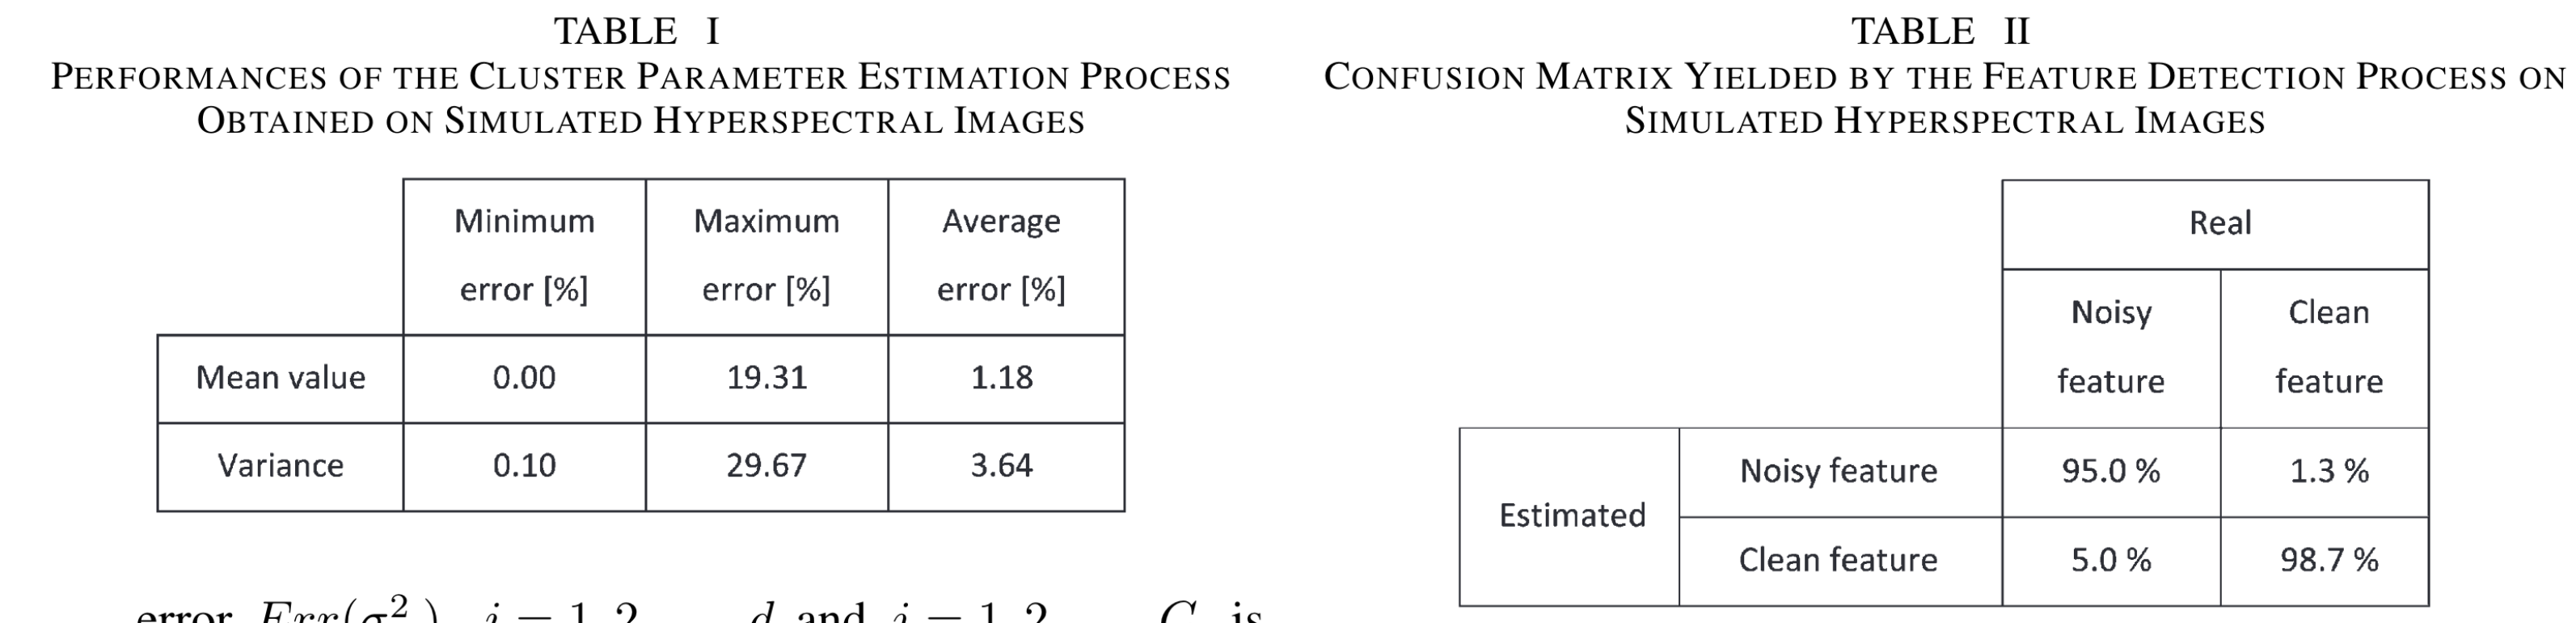
\includegraphics[width=1\linewidth]{paoli_tables.png}
    \captionsetup{labelformat=simple, labelsep=colon, font=tiny, labelfont={color=gray,bf}}
    \caption{\textbf{Performance Metrics and Confusion Matrix for Clustering Hyperspectral Images Using MOPSO} Table I shows the performance of the cluster parameter estimation process, with minimum, maximum, and average error percentages and their variances. Table II presents the confusion matrix for the feature detection process, illustrating the classification accuracy of noisy and clean features in simulated hyperspectral images. (Paoli et al.)\cite{amigoHyperspectralImageAnalysis2015}}
    \label{fig:paoli_tables}
\end{figure}
\vspace{-0.5cm} % Adjust this value as needed to reduce the space
\begin{itemize}
    \item Alajlan, N., et al. (2012). Fusion of Supervised and Unsupervised Learning for Improved Classification of Hyperspectral Images. \textit{IEEE Transactions on Geoscience and Remote Sensing}, 50(8), 2851-2863. \href{https://consensus.app/papers/fusion-supervised-learning-improved-classification-alajlan/7f6e4675e84c5be298365122c11f6858/?utm_source=chatgpt}{\color{blue}{DOI: 10.1109/TGRS.2011.2172168}}
    {\color{gray}Introduces a novel framework combining supervised and unsupervised learning for hyperspectral image classification using support vector machines and fuzzy C-means clustering.}

    \item Bevilacqua, V., Berthoumieu, Y. (2017). Unsupervised Band Selection via Multi-feature Information-maximization Clustering. \textit{IEEE Transactions on Geoscience and Remote Sensing}, 55(2), 1040-1050. \href{https://consensus.app/papers/unsupervised-band-selection-multifeature-bevilacqua/d351f61026a35f8f9463f907b37e7d27/?utm_source=chatgpt}{\color{blue}{DOI: 10.1109/TGRS.2016.2626904}}
    {\color{gray}Treats hyperspectral band selection as a clustering problem, maximizing mutual information between data features and cluster assignments.}
\end{itemize}
\end{frame}

\begin{frame}{Landmark Papers (2/3)}
\footnotesize
\begin{itemize}
    \item Lee, S., Crawford, M.M. (2004). Hierarchical Clustering Approach for Unsupervised Image Classification of Hyperspectral Data. \textit{IEEE Transactions on Geoscience and Remote Sensing}, 42(12), 2675-2686. \href{https://consensus.app/papers/clustering-approach-image-classification-data-lee/7e01c6a70ab75aae8291e5d179d7374e/?utm_source=chatgpt}{\color{blue}{DOI: 10.1109/TGRS.2004.834614}}
    {\color{gray}Proposes a multistage hierarchical clustering technique, combining local and global segmentors for hyperspectral data classification.}

    \item Kiran, B.R., et al. (2016). Unsupervised Clustering of Hyperspectral Images of Brain Tissues by Hierarchical Non-negative Matrix Factorization. \textit{IEEE Transactions on Biomedical Engineering}, 63(9), 1834-1842. \href{https://consensus.app/papers/unsupervised-clustering-hyperspectral-images-brain-kiran/0612dc71f71f5118a9467490481ad6be/?utm_source=chatgpt}{\color{blue}{DOI: 10.1109/TBME.2015.2509484}}
    {\color{gray}Applies hierarchical non-negative matrix factorization for unsupervised clustering of brain tissue hyperspectral images.}

    \item Datta, S., et al. (2012). Clustering Based Band Selection for Hyperspectral Images. \textit{IEEE Transactions on Geoscience and Remote Sensing}, 50(11), 4237-4248. \href{https://consensus.app/papers/clustering-based-band-selection-images-datta/78493a3d39e8521db170ba8cad157c2a/?utm_source=chatgpt}{\color{blue}{DOI: 10.1109/TGRS.2012.2186344}}
    {\color{gray}Presents an unsupervised band selection method using DBSCAN clustering, focusing on reducing redundancy among spectral bands.}

    \item Paoli, M., et al. (2009). Clustering of Hyperspectral Images Based on Multi-objective Particle Swarm Optimization. \textit{IEEE Transactions on Geoscience and Remote Sensing}, 47(12), 4175-4189. \href{https://consensus.app/papers/clustering-hyperspectral-images-based-multiobjective-paoli/76e19f51eed85904a08c9b811f014d8f/?utm_source=chatgpt}{\color{blue}{DOI: 10.1109/TGRS.2009.2025099}}
    {\color{gray}Uses multi-objective particle swarm optimization to simultaneously estimate class statistical parameters, select discriminative bands, and determine the number of data classes.}
\end{itemize}
\end{frame}

\begin{frame}{Landmark Papers (3/3)}
\footnotesize
\begin{itemize}
    \item Bidhendi, S.R., et al. (2007). Material Classification of Hyperspectral Images Using Unsupervised Fuzzy Clustering Methods. \textit{Journal of Applied Remote Sensing}, 1(1), 011510. \href{https://consensus.app/papers/classification-hyperspectral-images-using-unsupervised-bidhendi/ac0b5a2ecb8958599373f4d51686fba2/?utm_source=chatgpt}{\color{blue}{DOI: 10.1117/1.2794359}}

    {\color{gray}Classifies materials in hyperspectral images using fuzzy C-means and fuzzy relational clustering methods, focusing on creating clusters based on the data itself.}

    \item Habermann, J.D., et al. (2022). Unsupervised Cluster-Wise Hyperspectral Band Selection for Classification. \textit{IEEE Transactions on Geoscience and Remote Sensing}, 60, 4104212. \href{https://consensus.app/papers/unsupervised-clusterwise-hyperspectral-band-selection-habermann/6429aafba4da503c91677e9a15644ff8/?utm_source=chatgpt}{\color{blue}{DOI: 10.1109/TGRS.2021.3137020}}

    {\color{gray}Proposes a new dimensionality reduction algorithm for hyperspectral images using a clustering approach for unsupervised band selection.}
\end{itemize}
\end{frame}

\subsection{HSI + }
\begin{frame}{HSI + Medical Diagnostics (1/2)}
\footnotesize
\begin{figure}
    \centering
    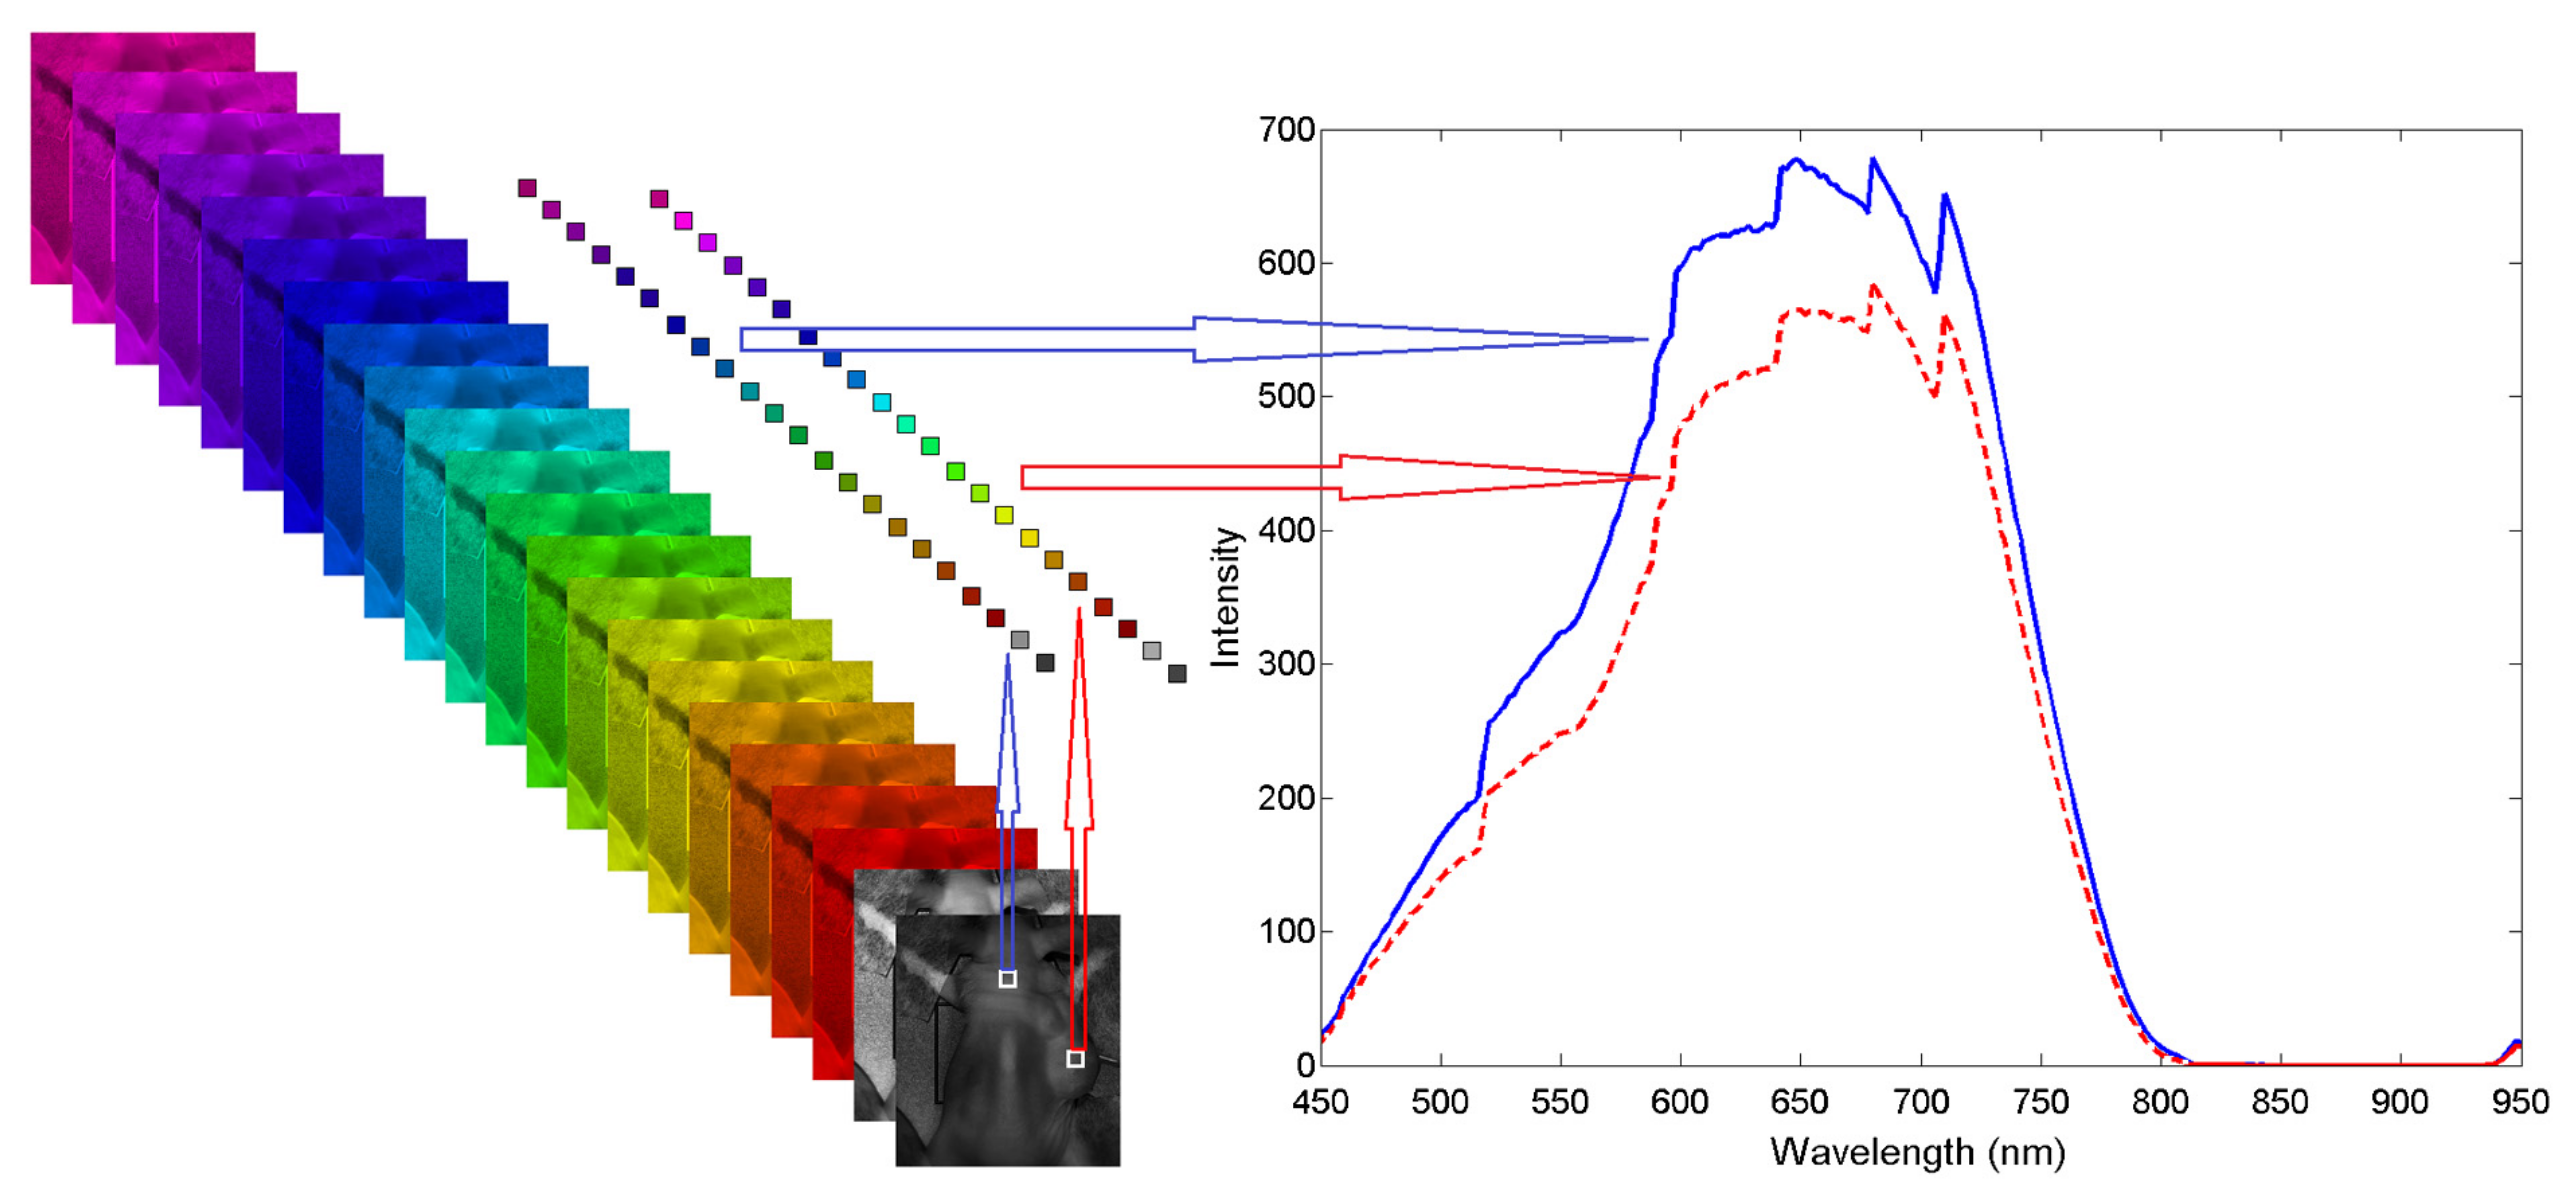
\includegraphics[width=0.61\linewidth]{akabari_figure.png}
    \captionsetup{labelformat=simple, labelsep=colon, font=tiny, labelfont={color=gray,bf}}
    \caption{\textbf{Hyperspectral Images of a Nude Mouse} The left side shows the hyperspectral image cube, while the right side presents spectral graphs of cancer (dashed line) and normal (solid line) tissue, depicting normalized reflectance across wavelengths.)\cite{akbariHyperspectralImagingQuantitative2012}}
    \label{fig:akabari_figure}
\end{figure}
\vspace{-0.5cm} % Adjust this value as needed to reduce the space
\begin{itemize}
    \item Lu, G., Fei, B. (2014). Medical Hyperspectral Imaging: A Review. \textit{Journal of Biomedical Optics}, 19(1), 010901. \href{https://www.spiedigitallibrary.org/journals/journal-of-biomedical-optics/volume-19/issue-01/010901/Medical-hyperspectral-imaging-a-review/10.1117/1.JBO.19.1.010901.full}{\color{blue}{DOI: 10.1117/1.JBO.19.1.010901}}

    {\color{gray}This review covers the applications of hyperspectral imaging in medical fields, particularly in disease diagnosis and image-guided surgery. It emphasizes the benefits of HSI in providing non-invasive diagnostic capabilities.}

    \item Ortega, S., Fabelo, H., Iakovidis, D.K., et al. (2018). Detecting Brain Tumor Slides Using Hyperspectral Imaging. \textit{IEEE Transactions on Biomedical Engineering}, 65(11), 2580-2588. \href{https://consensus.app/papers/detecting-brain-tumor-slides-using-imaging-ortega/4e764c565e1852f8867aabec0ca253f4/?utm_source=chatgpt}{\color{blue}{DOI: 10.1109/TBME.2018.2847218}}

    {\color{gray}Shows promise in automatically detecting high-grade brain tumors in pathological slides using spectral libraries and classification algorithms.}
\end{itemize}
\end{frame}

\begin{frame}{HSI + Medical Diagnostics (2/2)}
\footnotesize
\begin{itemize}
    \item Akbari, H., et al. (2012). Hyperspectral Imaging for Prostate Cancer Detection. \textit{IEEE Transactions on Biomedical Engineering}, 59(4), 949-952. \href{https://consensus.app/papers/hyperspectral-imaging-analysis-prostate-cancer-akbari/867fee31d50759d8a8ebe58fcc5cd750/?utm_source=chatgpt}{\color{blue}{DOI: 10.1109/TBME.2012.2189882}}

    {\color{gray}Utilizes hyperspectral imaging to detect prostate cancer by analyzing spectral signatures of cancerous and normal tissues.}

    \item Schellinger, P.D., et al. (1999). Standardized Stroke MRI: Comparison of Hyperacute Stroke Imaging Protocols. \textit{Stroke}, 30(4), 765-768. \href{https://consensus.app/papers/standardized-stroke-comparison-hemorrhage-schellinger/8fbc8c749c435c8e94e7af9de90a78aa/?utm_source=chatgpt}{\color{blue}{DOI: 10.1161/01.STR.30.4.765}}

    {\color{gray}Explores the effectiveness of MRI with hyperspectral imaging for assessing hyperacute intracerebral hemorrhage (ICH) and ischemic strokes.}

    \item Fiebach, J.B., et al. (2004). Stroke Magnetic Resonance Imaging is Accurate in Hyperacute Stroke: A Cohort Study. \textit{Stroke}, 35(2), 502-506. \href{https://consensus.app/papers/stroke-magnetic-resonance-imaging-accurate-hyperacute-fiebach/f5f34a7ddc415e8b88f3c4b51ee76d5c/?utm_source=chatgpt}{\color{blue}{DOI: 10.1161/01.STR.0000114871.19735.23}}

    {\color{gray}Investigates the accuracy of MRI with hyperspectral imaging in diagnosing hyperacute strokes.}

    \item Ortega, S., et al. (2020). Hyperspectral Imaging in Pathology: A Review. \textit{Journal of Pathology Informatics}, 11, 35. \href{https://consensus.app/papers/imaging-pathology-review-invited-ortega/da0cdf35f01d556d80c0c17d41bacee3/?utm_source=chatgpt}{\color{blue}{DOI: 10.4103/jpi.jpi\_16\_20}}

    {\color{gray}Reviews the application of hyperspectral imaging in pathology, enhancing the detection of various cancers and other diseases.}
\end{itemize}
\end{frame}


\begin{frame}{HSI + EEG/BCI (1/2)}
\footnotesize
\begin{figure}
    \centering
    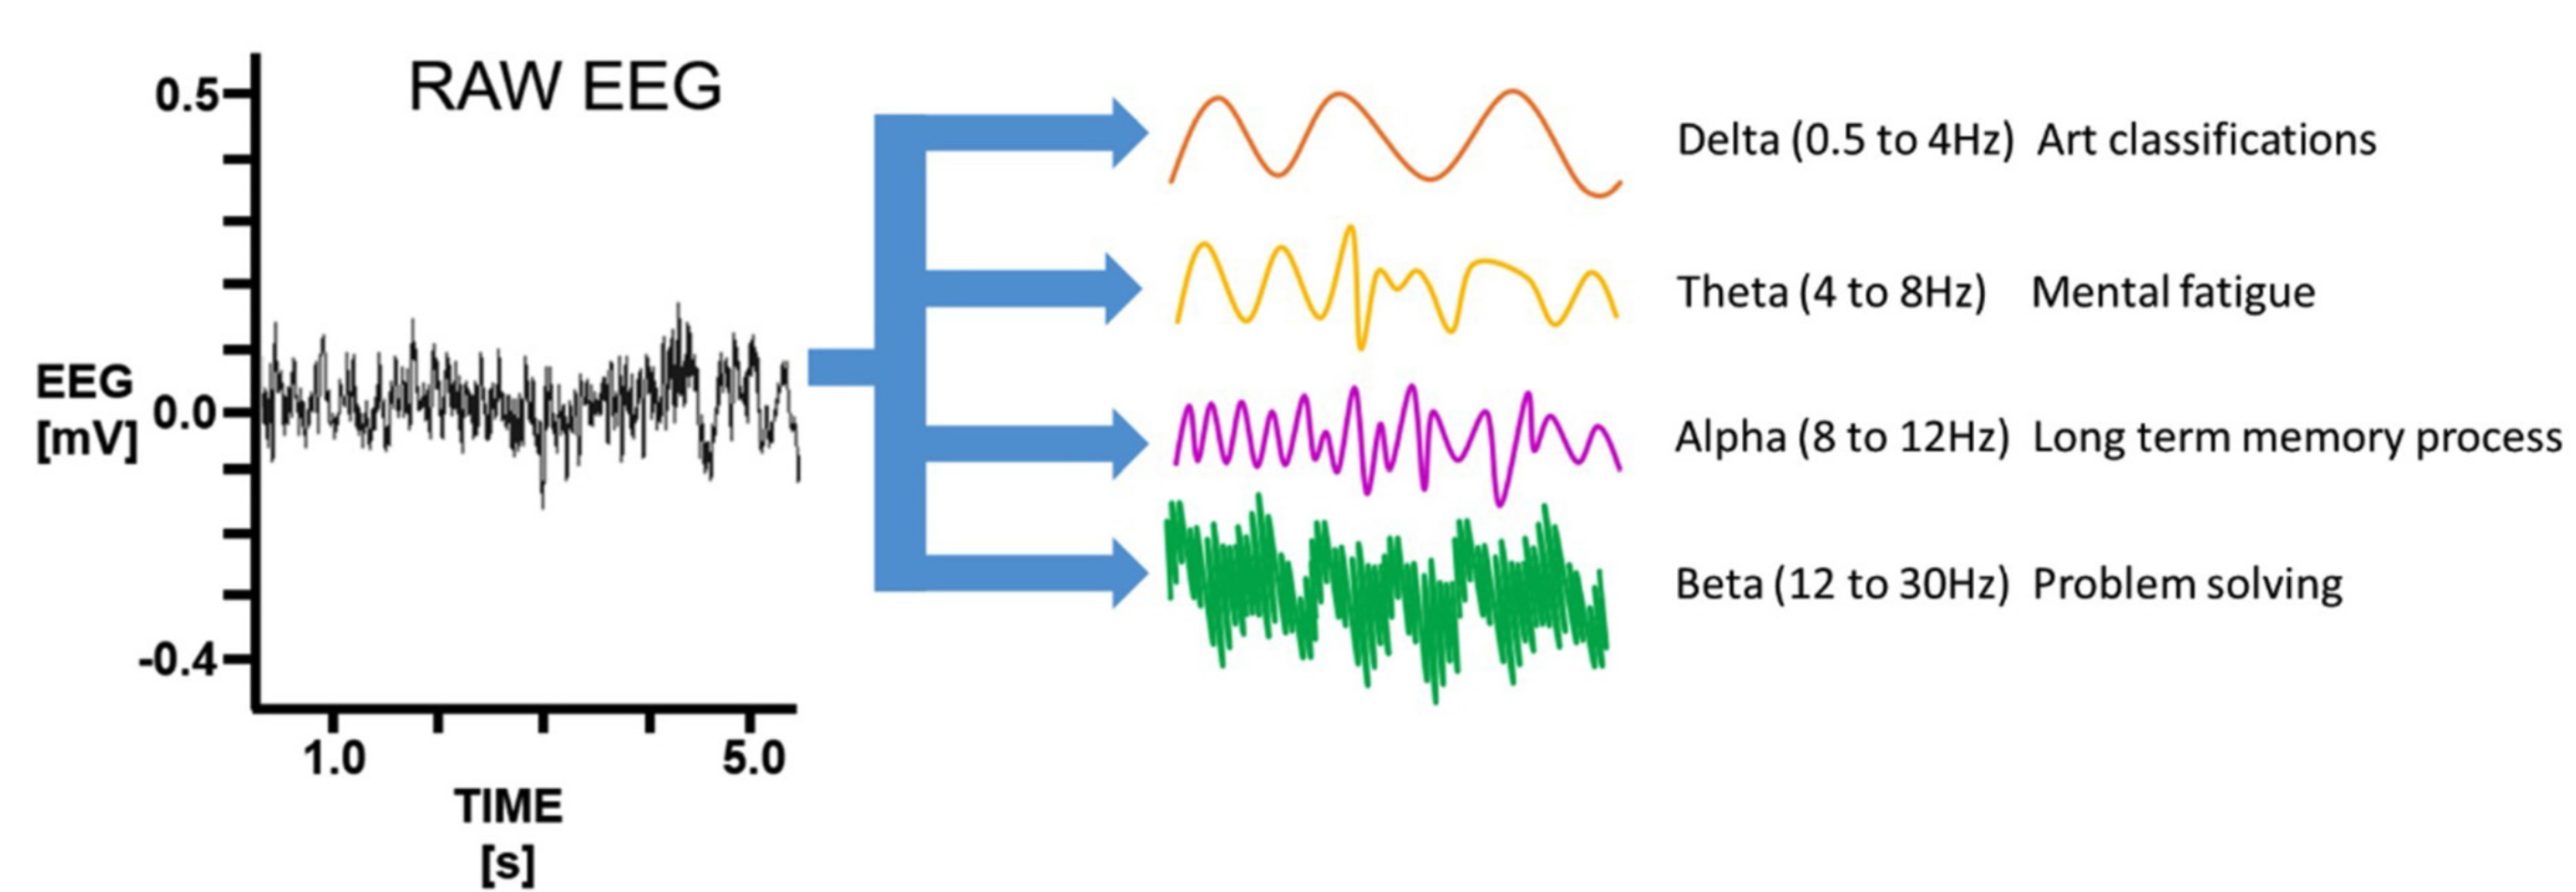
\includegraphics[width=0.62\linewidth]{robotor_figure.png}
    \captionsetup{labelformat=simple, labelsep=colon, font=tiny, labelfont={color=gray,bf}}
    \caption{\textbf{EEG Frequency Bands and Brain Activity} The schematic shows the raw EEG trace decomposed into delta (0.5 to 4 Hz), theta (4 to 8 Hz), alpha (8 to 12 Hz), and beta (12 to 30 Hz) waves, each associated with different brain functions such as art classification, mental fatigue, memory processing, and problem solving.)\cite{portillo-laraMindGapStateoftheart2021}}
    \label{fig:robotor_figure}
\end{figure}
\vspace{-0.5cm} % Adjust this value as needed to reduce the space
\begin{itemize}
    \item Ahn, M., Jun, S.C. (2017). Multi-modal Integration of EEG and fNIRS for Brain-Computer Interface Applications. \textit{IEEE Transactions on Neural Systems and Rehabilitation Engineering}, 25(1), 142-153. \href{https://consensus.app/papers/multimodal-integration-eegfnirs-braincomputer-ahn/7783794289e4511c90f93959f447cf57/?utm_source=chatgpt}{\color{blue}{DOI: 10.1109/TNSRE.2016.2557239}}

    {\color{gray}Combining EEG with functional near-infrared spectroscopy (fNIRS) to enhance BCI performance by supplementing limitations of single modality.}

    \item Hasan, M.K., Khan, M.J., Mishra, S. (2020). Computationally Efficient Method for Hybrid EEG-fNIRS Based BCI Systems. \textit{IEEE Transactions on Biomedical Engineering}, 67(10), 2924-2931. \href{https://consensus.app/papers/computationally-efficient-method-hybrid-eegfnirs-based-hasan/1d25bad4992156eab4b1259e11f70aff/?utm_source=chatgpt}{\color{blue}{DOI: 10.1109/TBME.2020.2970158}}

    {\color{gray}Uses Pearson product-moment correlation for channel selection in hybrid EEG-fNIRS systems, improving computational efficiency and classification accuracy.}
\end{itemize}
\end{frame}

\begin{frame}{HSI + EEG/BCI (2/2)}
\footnotesize
\begin{itemize}
    \item Corsi, M.C., et al. (2017). Integrating EEG and MEG Signals to Improve Motor Imagery Classification. \textit{Journal of Neural Engineering}, 14(5), 056010. \href{https://consensus.app/papers/integrating-signals-improve-motor-imagery-corsi/952af2ce3ef55c94a5fcedf7fbb7ffbe/?utm_source=chatgpt}{\color{blue}{DOI: 10.1088/1741-2552/aa87d2}}

    {\color{gray}Combines EEG and MEG signals to enhance motor imagery classification in BCIs, showing improved performance compared to single-modality systems.}

    \item Portillo-Lara, R., et al. (2021). Wearable EEG Technologies for Non-Invasive BCIs: State of the Art and Future Directions. \textit{IEEE Reviews in Biomedical Engineering}, 14, 84-97. \href{https://consensus.app/papers/mind-stateoftheart-technologies-applications-eegbased-portillolara/b5f98d6cf787507cb6ffcae48ff8a313/?utm_source=chatgpt}{\color{blue}{DOI: 10.1109/RBME.2020.2970354}}

    {\color{gray}Reviews advances in wearable EEG technology for non-invasive BCIs, focusing on real-world applications and novel electrode interfaces.}

    \item Jiang, X., et al. (2014). A Brain-Computer Interface Based on Hybrid EEG and EOG Signals for Detecting User Intent. \textit{IEEE Transactions on Neural Systems and Rehabilitation Engineering}, 22(2), 321-327. \href{https://consensus.app/papers/braincomputer-interface-based-signals-jiang/24a2ced8418855838524bb9921769bae/?utm_source=chatgpt}{\color{blue}{DOI: 10.1109/TNSRE.2013.2294695}}

    {\color{gray}Combines EEG with electrooculography (EOG) signals to enhance BCI control, improving target selection accuracy and flexibility.}
\end{itemize}
\end{frame}

\begin{frame}{HSI + DL (1/3)}
\footnotesize
\begin{itemize}
    \item Khan, M.J., et al. (2020). Trends in Deep Learning for Medical Hyperspectral Image Analysis. \textit{IEEE Journal of Biomedical and Health Informatics}. \href{https://consensus.app/papers/trends-deep-learning-medical-hyperspectral-image-khan/df926a1f23575de086631c2a78a80c3b/?utm_source=chatgpt}{\color{blue}{DOI: 10.1109/JBHI.2020.3005904}}

    {\color{gray}Discusses the application of deep learning techniques for classification, segmentation, and detection in medical hyperspectral images.}

    \item Cui, H., et al. (2022). Deep Learning for Medical Hyperspectral Images: A Systematic Review. \textit{IEEE Journal of Biomedical and Health Informatics}. \href{https://consensus.app/papers/deep-learning-medical-hyperspectral-images-review-cui/f417345410c95b21b20d7aba8a773f9b/?utm_source=chatgpt}{\color{blue}{DOI: 10.1109/JBHI.2022.3140152}}

    {\color{gray}A systematic review highlighting the application of deep learning in medical diagnostics, combining spectral and spatial information.}

    \item Yang, Y., et al. (2018). Image Classification with Deep Learning Models for Remote Sensing. \textit{IEEE Transactions on Geoscience and Remote Sensing}. \href{https://consensus.app/papers/image-classification-with-deep-learning-models-yang/26245f0c21415e8e85c9e8b0a5085376/?utm_source=chatgpt}{\color{blue}{DOI: 10.1109/TGRS.2018.2845367}}

    {\color{gray}Discusses the use of deep learning models like 2-D and 3-D CNNs for hyperspectral image classification.}

    \item Zhou, J., Prasad, S. (2020). Advances in Deep Learning for Hyperspectral Image Analysis. \textit{IEEE Journal of Selected Topics in Applied Earth Observations and Remote Sensing}, 13, 711-725. \href{https://consensus.app/papers/advances-deep-learning-hyperspectral-image-zhou/17caa3d1f836545db0a099a1d43e708e/?utm_source=chatgpt}{\color{blue}{DOI: 10.1109/JSTARS.2020.2987548}}

    {\color{gray}Explores transfer learning and semi-supervised learning approaches for hyperspectral image analysis to address the scarcity of labeled data.}
\end{itemize}
\end{frame}

\begin{frame}{HSI + DL (2/2)}
\footnotesize
\begin{itemize}
    \item Wang, L., et al. (2021). Review of Deep Learning Used in Image Analysis for Agriculture. \textit{Computers and Electronics in Agriculture}, 175, 105561. \href{https://consensus.app/papers/review-learning-used-image-analysis-agriculture-wang/68e0e3e870035e8eb2698f31d1c8c364/?utm_source=chatgpt}{\color{blue}{DOI: 10.1016/j.compag.2020.105561}}

    {\color{gray}Reviews the application of deep learning in agricultural hyperspectral images, focusing on crop health, disease detection, and quality attribute analysis.}

    \item Chen, Y., et al. (2016). Feature Extraction and Classification of Hyperspectral Images with Deep Convolutional Neural Networks. \textit{IEEE Journal of Selected Topics in Applied Earth Observations and Remote Sensing}, 9(9), 4600-4613. \href{https://consensus.app/papers/feature-extraction-classification-hyperspectral-images-chen/966c8029a2295c7b8f9cb04e4be39ad9/?utm_source=chatgpt}{\color{blue}{DOI: 10.1109/JSTARS.2016.2619742}}

    {\color{gray}Uses advanced deep learning techniques, including 3-D CNNs and recurrent neural networks (RNNs), for feature extraction and classification.}

    \item Liu, B., et al. (2021). Deep Multiview Learning for Hyperspectral Image Classification. \textit{IEEE Transactions on Neural Networks and Learning Systems}, 32(5), 1941-1954. \href{https://consensus.app/papers/deep-multiview-learning-hyperspectral-image-liu/9eb84004885252c1ae9b997d560673ca/?utm_source=chatgpt}{\color{blue}{DOI: 10.1109/TNNLS.2020.2997472}}

     {\color{gray}Introduces deep multiview learning and dimensionality reduction techniques for hyperspectral image classification.}
\end{itemize}
\end{frame}

\section{Benchmark Datasets}
\begin{frame}{Benchmark Datasets in HSI - Part 1}
\small
\begin{figure}
    \centering
    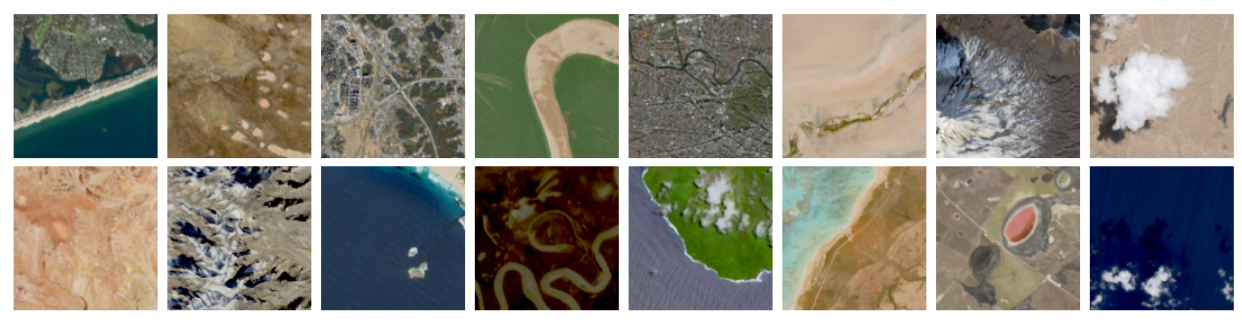
\includegraphics[width=1\linewidth]{HySpecNet_example.png}
    \captionsetup{labelformat=simple, labelsep=colon, font=tiny, labelfont={color=gray,bf}}
    \caption{True color representations of example images from our proposed HySpecNet-11k dataset. Red, green, and blue channels are extracted from EnMAP bands 43, 28, and 10 at wavelengths 634.919 nm, 550.525 nm, and 463.584 nm, respectively.\cite{fuchsHySpecNet11kLargeScaleHyperspectral2023}}
    \label{fig:HySpecNet-example}
\end{figure}
\vspace{-1cm} % Adjust this value as needed to reduce the space
\begin{table}[]
    \centering
    \begin{tabular}{|p{4.5cm}|p{6cm}|p{0.5cm}|}
        \hline
        \textbf{Title (DOI)} & \textbf{Description} & \textbf{Cite} \\ \hline
        HySpecNet-11k: A Large-Scale Hyperspectral Dataset for Image Compression and Unsupervised Learning \newline \href{https://consensus.app/papers/hyspecnet11k-largescale-hyperspectral-dataset-fuchs/86b52e4fcd0c50f6b4c0da950c6e4c11/?utm_source=chatgpt}{\color{blue}10.1109/TGRS.2023.3155567} & This large-scale dataset consists of 11,483 non-overlapping image patches, each with 224 spectral bands, designed for hyperspectral image compression and unsupervised learning tasks. & \cite{fuchsHySpecNet11kLargeScaleHyperspectral2023} \\ \hline
    \end{tabular}
\end{table}
\end{frame}

\begin{frame}{Benchmark Datasets in HSI - Part 1 (Contd.)}
\small
\begin{figure}
    \centering
    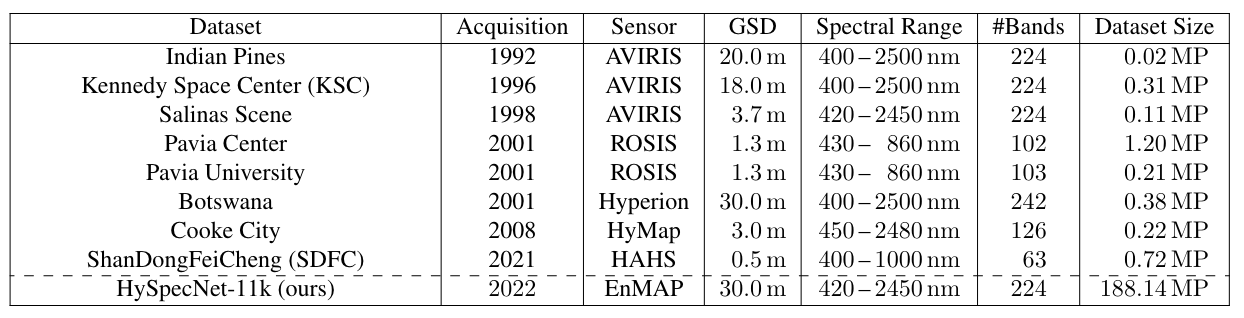
\includegraphics[width=1\linewidth]{HySpecNet_table.png}
    \captionsetup{labelformat=simple, labelsep=colon, font=tiny, labelfont={color=gray,bf}}
    \caption{A summary of publicly available hyperspectral benchmark datasets and their characteristics.\cite{fuchsHySpecNet11kLargeScaleHyperspectral2023}}
    \label{fig:HySpecNet-example}
\end{figure}
\vspace{-0.8cm} % Adjust this value as needed to reduce the space
\begin{table}[]
    \centering
    \begin{tabular}{|p{4.5cm}|p{6cm}|p{0.5cm}|}
        \hline
        \textbf{Title (DOI)} & \textbf{Description} & \textbf{Cite} \\ \hline
        HySpecNet-11k: A Large-Scale Hyperspectral Dataset for Image Compression and Unsupervised Learning \newline \href{https://consensus.app/papers/hyspecnet11k-largescale-hyperspectral-dataset-fuchs/86b52e4fcd0c50f6b4c0da950c6e4c11/?utm_source=chatgpt}{\color{blue}10.1109/TGRS.2023.3155567} & This large-scale dataset consists of 11,483 non-overlapping image patches, each with 224 spectral bands, designed for hyperspectral image compression and unsupervised learning tasks. & \cite{fuchsHySpecNet11kLargeScaleHyperspectral2023} \\ \hline
    \end{tabular}
\end{table}
\end{frame}

\begin{frame}{Benchmark Datasets in HSI - Part 2}
\small
\begin{figure}
    \centering
    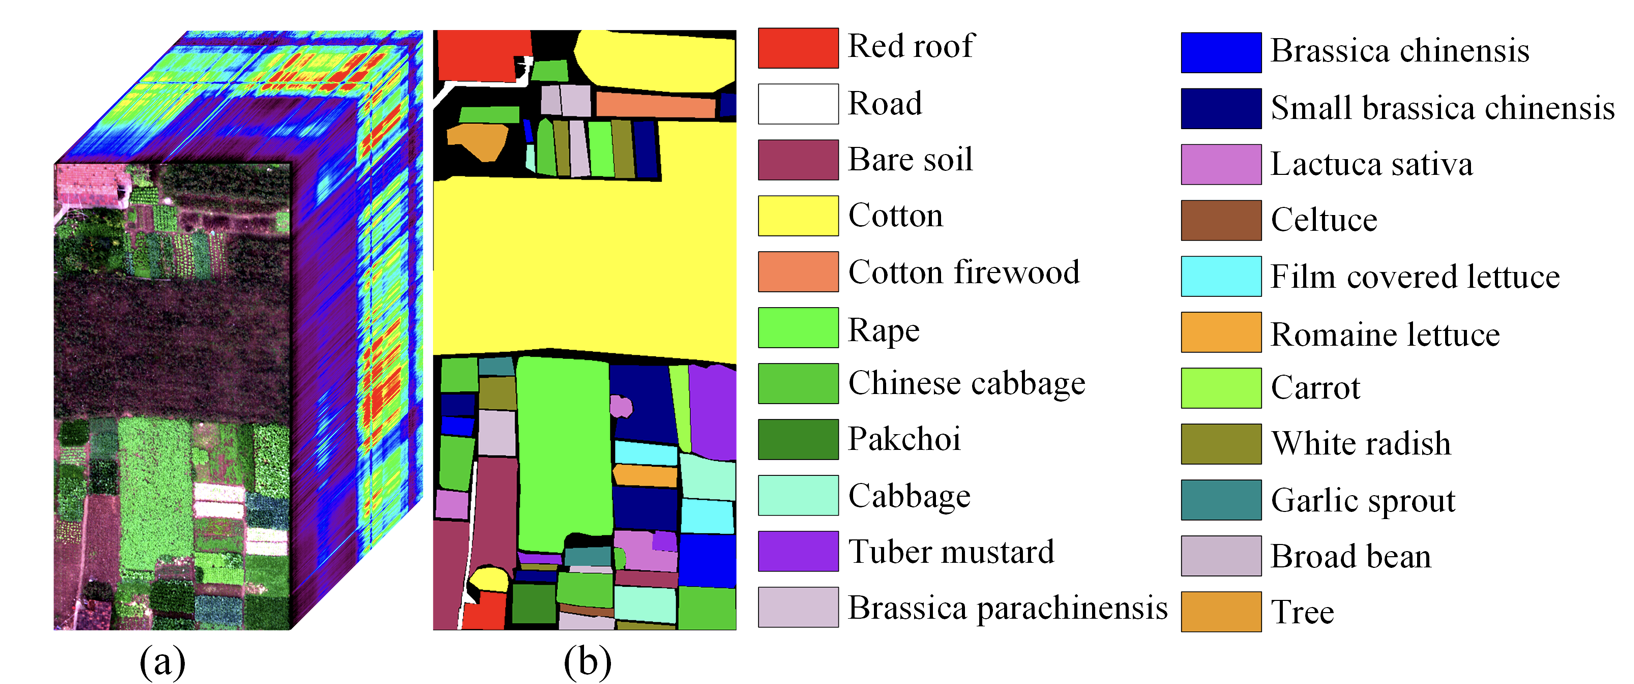
\includegraphics[width=0.62\linewidth]{WHU-Hi.png}
    \captionsetup{labelformat=simple, labelsep=colon, font=tiny, labelfont={color=gray,bf}}
    \caption{The WHU-Hi-HongHu dataset. (a) Image cube. (b) Ground-truth image.\cite{huWHUHiUAVborneHyperspectral}}
    \label{fig:WHU-Hi}
\end{figure}
\vspace{-1cm} % Adjust this value as needed to reduce the space
\begin{table}[]
    \centering
    \begin{tabular}{|p{4.5cm}|p{6cm}|p{0.5cm}|}
        \hline
        \textbf{Title (DOI)} & \textbf{Description} & \textbf{Cite} \\ \hline
        WHU-Hi: A UAV-borne Hyperspectral Image Dataset for Classification \newline \href{https://consensus.app/papers/whuhi-uavborne-resolution-benchmark-datasets-image-hu/c738ddb273815adda3d8fadfcd4f0192/?utm_source=chatgpt}{\color{blue}10.1109/TGRS.2020.2983299} & [RS] The Wuhan UAV-borne hyperspectral image dataset provides high spectral and spatial resolution data for hyperspectral image classification. & \cite{huWHUHiUAVborneHyperspectral} \\ \hline
    \end{tabular}
\end{table}
\end{frame}

\begin{frame}{Benchmark Datasets in HSI - Part 3}
\small
\begin{figure}
    \centering
    \begin{columns}[T] % Align columns at the top
        % Left column with the image
        \begin{column}{0.38\textwidth}
            \centering
            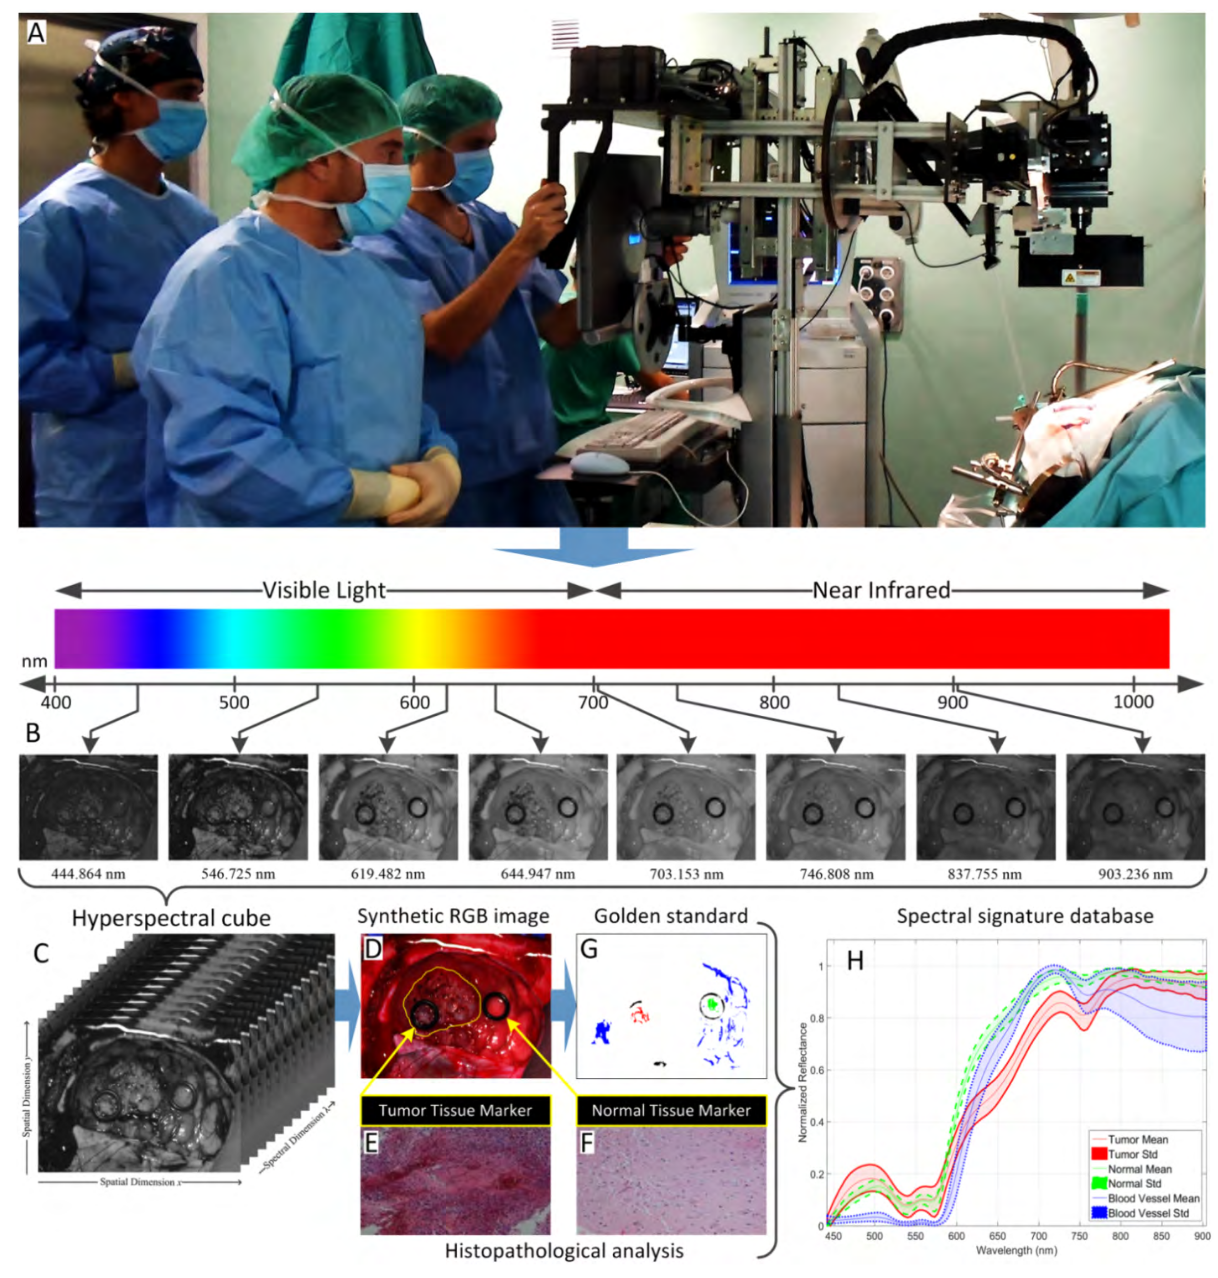
\includegraphics[width=0.8\linewidth]{In-Vivo.png}
        \end{column}
        % Right column with the caption
        \begin{column}{0.62\textwidth}
            \captionsetup{labelformat=simple, labelsep=colon, font=tiny, labelfont={color=gray,bf}}
            \caption{In-vivo HS brain surface acquisition procedure. (a) Hyperspectral acquisition system being used during the acquisition process in a neurosurgical operation. (b) Hyperspectral images acquired with the acquisition system at different wavelengths from a patient affected by a glioblastoma tumor. (c) HSI data cube. (d) RGB image generated from the HS cube with the tumor tissue marker (left) and the normal tissue marker (right) placed on the brain surface. (e) and (f) Histopathological images of the tumor tissue sample (glioblastoma) and normal tissue sample respectively. (g) Gold standard map where certain pixels have been labeled in four different classes: normal brain tissue (green), tumor tissue (red), blood vessel (blue) and background (black). (h) Average and standard deviation (Std) of the pre-processed spectral signatures of tumor tissue, normal tissue and blood vessel labeled pixels, represented in red, green and blue color respectively.\cite{fabeloInVivoHyperspectralHuman2019}}
        \end{column}
    \end{columns}
    \label{fig:In-Vivo}
\end{figure}
\vspace{-1cm} % Adjust this value as needed to reduce the space
\begin{table}[]
    \centering
    \begin{tabular}{|p{4.5cm}|p{6cm}|p{0.5cm}|}
        \hline
        \textbf{Title (DOI)} & \textbf{Description} & \textbf{Cite} \\ \hline
        In-Vivo Hyperspectral Human Brain Image Database \newline \href{https://consensus.app/papers/invivo-hyperspectral-human-brain-image-database-brain-fabelo/14753e1e2ea15718be292f660ad9ec53/?utm_source=chatgpt}{\color{blue}10.1109/TMI.2019.2926947} & [BME] Developed for brain cancer detection, this dataset includes hyperspectral images of human brain tissues acquired during neurosurgery. & \cite{fabeloInVivoHyperspectralHuman2019} \\ \hline
    \end{tabular}
\end{table}
\end{frame}

\begin{frame}{Benchmark Datasets in HSI - Part 4}
\small
\begin{table}[]
    \centering
    \begin{tabular}{|p{4.5cm}|p{6cm}|p{0.5cm}|}
        \hline
        \textbf{Title (DOI)} & \textbf{Description} & \textbf{Cite} \\ \hline
        Benchmark for Hyperspectral Unmixing Algorithm Evaluation \newline \href{https://consensus.app/papers/benchmark-hyperspectral-unmixing-algorithm-evaluation-paura/46070bf6345059e99d77d14e4dadef27/?utm_source=chatgpt}{\color{blue}10.1109/JSTARS.2023.3176657} & [RS] This dataset includes several hyperspectral images with ground truths for testing hyperspectral unmixing algorithms. & \cite{pauraBenchmarkHyperspectralUnmixing2023} \\ \hline
        Microscopic Hyperspectral Image Analysis: Datasets for Cell and Microplastics Detection \newline \href{https://consensus.app/papers/microscopic-hyperspectral-image-analysis-deep-learning-chen/aaa2e55a0cd357e6bd6615d6683789c3/?utm_source=chatgpt}{\color{blue}10.1109/TMI.2020.2975663} & [Mixed] Two benchmark datasets of cells and microplastics are used for cell classification and microplastics detection. & \cite{chenMicroscopicHyperspectralImage2020} \\ \hline
    \end{tabular}
\end{table}
\end{frame}



\section{Software Packages}
\begin{frame}{Tools for Hyperspectral Image Analysis}
\small % Reducing font size
\begin{itemize}
    \item 
\includegraphics[height=1em]{matlab_icon.png} \textbf{HYPER-Tools} (Matlab)\cite{mobarakiHYPERToolsGraphicalUserfriendly2018}: Integrates spectral and spatial preprocessing with robust analysis and visualization capabilities. Ideal for exploratory data analysis and machine learning.  \href{https://www.hypertools.org}{\color{blue}Read more}
    \item 
\includegraphics[height=1em]{matlab2_icon.png} \textbf{Hyperspectral Image Analysis Toolbox}\cite{arzuaga-cruzMATLABToolboxHyperspectral2004}: Extends Matlab for processing imagery, focusing on environmental and biomedical applications. \href{https://consensus.app/papers/matlab-toolbox-hyperspectral-image-analysis-arzuagacruz/c1ab5fe0544557e7af3de5e2ed62250a/?utm_source=chatgpt}{\color{blue}Read more}
    \item 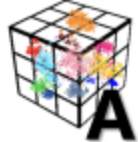
\includegraphics[height=1em]{qgis_icon.png} \textbf{AVHYAS Plugin for QGIS} \cite{lyngdohAVHYASFreeOpen2021}: Supports atmospheric correction and machine learning. Free and open-source. \href{https://sites.google.com/view/avhyas-sac-isro/home}{\color{blue}Read more}
    \item 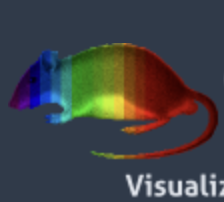
\includegraphics[height=1em]{generic_icon.png} \textbf{Gerbil} \cite{jordanNovelFrameworkInteractive2016}: An open-source framework for interactive visualization of hyperspectral data. \href{http://gerbilvis.org}{\color{blue}Read more}
    \item 
\includegraphics[height=1em]{envi_icon.png} \textbf{ENVI} \cite{xingHyperspectralImageAnalysis2001}: Commercial software for data pre-processing, analysis, and visualization. \href{hhttps://www.nv5geospatialsoftware.com/Products/ENVI}{\color{blue}Read more}
    \item 
\includegraphics[height=1em]{open_source_icon.png} \textbf{OpenSpyrit Ecosystem} \cite{benetimartinsOpenSpyritEcosystemOpen2023}: For hyperspectral single-pixel imaging, includes data acquisition and reconstruction tools. \href{https://github.com/openspyrit/spyrit}{\color{blue}Read more}
\end{itemize}
\end{frame}

\section{Conclusion}
\begin{frame}{Conclusion}
    \small
    \begin{itemize}
        \item Hyperspectral imaging combined with advanced unsupervised clustering techniques offers a powerful tool for detailed spectral analysis across various applications.
        \item Integration with EEG and BCI technologies provides enhanced capabilities for brain signal analysis, improving the accuracy and efficiency of these systems.
        \item The state-of-the-art methods, benchmark datasets, and ready software packages provide a solid foundation for further research and development in hyperspectral image analysis.
    \end{itemize}
\end{frame}

\section{Further Reading}
\begin{frame}{Further Reading}
    \frametitle{Access the Full Research Repo}
    For more detailed information, access our GitHub page:
    
    \vspace{1em} % Adds some vertical space
    
    \href{https://github.com/qqgjyx/CS-Group/blob/main/}{https://github.com/qqgjyx/CS-Group/blob/main/}
\end{frame}

\section{References}
\begin{frame}[allowframebreaks]{References}
\small
\bibliographystyle{IEEEtran}
\bibliography{HSI}
\end{frame}

\end{document}


